% master_thesis.tex
% -------------------------------------------------------------------------
%   Modern Minimalist Master Thesis Template - Robotics (SINDy)
% -------------------------------------------------------------------------
\documentclass[
    11pt,               % Standard font size
    a4paper,            % Paper size
    oneside,            % Print on one side (change to 'twoside' for binding)
    numbers=noenddot,   % Removes end dots in numbering (e.g. 1.1 not 1.1.)
    parskip=half,       % Adds space between paragraphs (modern look)
    listof=totoc,       % Adds Lists of Figures/Tables to TOC
    bibliography=totoc  % Adds Bibliography to TOC
]{scrreprt}

% --- Essential Packages ---
\usepackage[utf8]{inputenc}
\usepackage[T1]{fontenc}
\usepackage[english]{babel}
\usepackage{microtype}      % Improves character kerning (essential for 'classy' look)
\usepackage[margin=2.5cm, bindingoffset=1cm]{geometry} % Clean margins

\usepackage{scrhack} % listing issue
\usepackage{csquotes} % babel quote

% --- Fonts (Palatino for text, Euler for math - very readable) ---
\usepackage{newpxtext}      % Palatino-like font
\usepackage{newpxmath}      % Matching math font
\usepackage[scaled=0.9]{helvet} % Helvetica for sans-serif (headers)

% --- Mathematics & Robotics Specifics ---
\usepackage{amsmath}
\usepackage{mathtools}
\usepackage{bm}             % Bold math symbols (\bm{x})
\usepackage{siunitx}        % Correct unit formatting (e.g. \SI{5}{\meter\per\second})

% --- Graphics & Tables ---
\usepackage{graphicx}       % For including images
\usepackage{booktabs}       % Professional tables (no vertical lines)
\usepackage{float}          % Better float placement
\usepackage{subcaption}     % For sub-figures (a) (b)

% --- Algorithms & Code ---
\usepackage[ruled,vlined]{algorithm2e} % For pseudocode
\usepackage{listings}       % For Python/Matlab code
\usepackage{xcolor}

% --- Header & Footer Styling (Clean/Minimalist) ---
\usepackage[automark,headsepline]{scrlayer-scrpage}
\clearpairofpagestyles
\ihead{\headmark}
\ohead{\pagemark}
\pagestyle{scrheadings}

% --- Hyperlinks (Must be loaded last) ---
\usepackage[colorlinks=true, linkcolor=black, citecolor=blue, urlcolor=blue]{hyperref}

% --- Bibliography ---
\usepackage[style=ieee, backend=biber]{biblatex}
\addbibresource{references.bib}

% --- Tikz ---
\usepackage{tikz}
\usepackage{etoolbox}
\usetikzlibrary{positioning,matrix,backgrounds,calc,fit}


\pgfdeclarelayer{background}
\pgfdeclarelayer{foreground}
\pgfsetlayers{background,main,foreground}

\definecolor{sindynullgray}{RGB}{200,200,200}
\definecolor{sindyforces}{RGB}{196,78,82}
\definecolor{sindynewton}{RGB}{85,168,104}
\definecolor{sindylagrange}{RGB}{129,114,179}

\newcommand{\lb}{[}
\newcommand{\rb}{]}

% Define the sindy component as a node style
\tikzset{
    sindy label/.style={font=\tiny, text=black,minimum height=0pt},
    sindy component text/.style={
        rectangle,
        minimum width=10pt,
        minimum height=1.5cm,
        rounded corners=5pt,
        fill=none,
        draw=none,
        inner sep=0pt,
        outer sep=1pt,
        align=center,
    },
    with label/.style={label={[sindy label]above:#1}},
    deactivated opacity/.style={opacity=0.3},
    full opacity/.style={opacity=1.0},
    sindy solution/.style={
        rectangle,
        minimum width=6pt,
        minimum height=6pt,
        rounded corners=3pt,
        fill=sindynullgray,
        draw=none,
        inner sep=0pt,
        outer sep=0pt,
        align=center,
        opacity=0.3,
    },
    sindy component/.style={
        rectangle,
        minimum width=6pt,
        minimum height=10pt,
        rounded corners=3pt,
        fill=sindynullgray,
        draw=none,
        inner sep=0pt,
        outer sep=1pt,
        align=center,
        opacity=0.3,
    },
}

\tikzset{
    % Le style pour la "patate" : notre système physique réel
    system/.style={
        fill=gray!30, 
        draw=black, 
        thick,
        opacity=0.8
    },
    % Le style pour les fonctions candidates du catalogue
    catalog_function/.style={
        draw=blue!80, 
        fill=blue!20, 
        circle, 
        opacity=0.6,
        line width=1pt
    }
}

\definecolor{sindypreknowledge}{RGB}{196,78,82}
\definecolor{sindystandard}{RGB}{85,168,104}
\definecolor{sindysolutionexplicit}{RGB}{129,114,179}
\definecolor{sindysolutionimplicit}{RGB}{204,185,116}


% --- Custom Commands for SINDy ---
\newcommand{\TODO}[1]{\textcolor{red}{\textbf{TODO: #1}}}

% -------------------------------------------------------------------------
%   DOCUMENT BEGINS
% -------------------------------------------------------------------------
\begin{document}

% --- Title Page ---
\begin{titlepage}
    \centering
    \vspace*{2cm}
    
    {\scshape\LARGE University Name \par}
    \vspace{1.5cm}
    
    {\huge\bfseries Data-Driven Identification of Nonlinear Dynamics in Robotic Systems\par}
    \vspace{0.5cm}
    {\Large\itshape Application of the SINDy Algorithm\par}
    
    \vspace{2cm}
    
    {\Large \textbf{Your Name}\par}
    \vspace{1cm}
    {\large A thesis submitted in partial fulfillment of the requirements\\ for the degree of Master of Science in Robotics\par}
    
    \vspace{3cm}
    
    \begin{tabular}{rl}
        \textbf{Supervisor:} & Prof. Dr. Jane Doe \\
        \textbf{Co-Supervisor:} & Dr. John Smith
    \end{tabular}
    
    \vfill
    {\large \today \par}
\end{titlepage}

% --- Front Matter ---
\pagenumbering{roman} 

\chapter*{Abstract}
\addcontentsline{toc}{chapter}{Abstract}
Here you write the summary of your work. Since you are studying SINDy, you should mention the challenge of modeling complex robotic dynamics, the data collection process, and how sparse regression helped identify the governing equations.

\chapter*{Acknowledgements}
Thanks to the lab, the supervisor, and coffee.

\tableofcontents
\listoffigures
\listoftables

\clearpage
\pagenumbering{arabic} 

% -------------------------------------------------------------------------
%   MAIN CONTENT
% -------------------------------------------------------------------------

%Start with \chapter{} after it is normal \section \subsection stuff
\chapter{Methods}
\label{ch:methods}

This chapter details the working principles of the Sparse Identification of Nonlinear Dynamics (SINDy) algorithm and outlines our specific contributions to the method. 

SINDy is a data-driven framework designed to \textbf{identify} governing equations from data. It applies to nonlinear ordinary differential equations (ODEs), defined generally as in Eq.~\eqref{eq:ode} and \eqref{eq:ode:ex}, and can be extended to partial differential equations (PDEs) as shown in Eq.~\eqref{eq:pde} and \eqref{eq:pde:ex}:

\begin{equation}
    \left( u^{(k)}(t) = f_k(t, u) \right)_{k \in \mathbb{N}}
    \label{eq:ode}
\end{equation}

\begin{equation}
    \left( \partial^\alpha u(x) = f_\alpha(x, u) \right)_{\alpha \in \mathbb{N}^n}
    \label{eq:pde}
\end{equation}

\noindent where $\alpha = (\alpha_1, \dots, \alpha_n)$ is a multi-index, and $\partial^\alpha = \frac{\partial^{|\alpha|}}{\partial x_1^{\alpha_1} \dots \partial x_n^{\alpha_n}}$.

\noindent This formalism encompasses systems subjected to external forces:
\begin{equation}
    \left( u^{(k)}(t) = \mathcal{A}_k(u) + F_k(t) \right)_{k \in \mathbb{N}}
    \label{eq:ode:ex}
\end{equation}

\begin{equation}
    \left( \partial^\alpha u = \underbrace{\mathcal{A}_\alpha(u)}_{\text{Internal Dynamics}} + \underbrace{S_\alpha(x)}_{\text{External Forces}} \right)_{\alpha \in \mathbb{N}^n}
    \label{eq:pde:ex}
\end{equation}

\noindent To facilitate the understanding of the following sections, we will focus primarily on ODEs. We adopt the state-space formulation:
\begin{equation}
    \dot{\mathcal{X}}(t) = f(\mathcal{X}(t)) + F(t)
    \label{eq:system-dynamics}
\end{equation}
Note that while this resembles a matrix formulation, $f$ represents a general non-linear vector function, not necessarily a linear transformation. Although the generalization to PDEs is conceptually similar, we restrict our analysis to ODEs for clarity.

\section{Core SINDy Principle}
\textit{\textcolor{gray}{[Background - State of the Art]}}

SINDy, as developed by Brunton et al.\cite{bruntonDiscoveringGoverningEquations2016}, relies on the decomposition of dynamics into linearly dependent components. In order to achieve this we assume that the dynamics will lies inside a set of predetermined non-linear and linear function (eg. $(cos,sin,\cdot^2,\sqrt{\cdot},\dots)$). This function catalog $\boldsymbol{\Theta} = (f_1(\mathcal{X}),f_2(\mathcal{X}),\dots,f_k(\mathcal{X}))$will bridge the gap between linear ODEs and non-linear ones. A particuliar attention should be made during the selection of the catalog. \TODO{link this with concerned chapter}

It can be noted that in the next subsection we make the distinction between the different coordinate when applying a catalog function for ease of comprehension we introduce the following subscript notation $cos_2(\mathcal{X}(t))=cos(x_2(t))$.

Since SINDy is a data-driven method instead of relying on theoretical formulation, we manipulate discrete state-space matrices $\boldsymbol{X}$. In order to streamline comprehension in the next chapters, we introduce right now the concept of \textsc{symbol matrix} $\boldsymbol{X}_t$:
\begin{equation}
    \boldsymbol{X}_{t} = \begin{bmatrix}
        x_1(t) & x_2(t) & \cdots & x_n(t) \\
        \dot{x}_1(t) & \dot{x}_2(t) & \cdots & \dot{x}_n(t) \\
        \ddot{x}_1(t) & \ddot{x}_2(t) & \cdots & \ddot{x}_n(t)
    \end{bmatrix}
\end{equation}
\noindent We don't need to go past the second derivative (acceleration) in all our next study. The set of sample $\boldsymbol{X}=(\boldsymbol{X}_{t_k})_{k\in [1,\dots,m]}$, will be considered as our input in all next study.

The next step is now to populate the experiment matrix $\boldsymbol{\Theta}(\boldsymbol{X})$ with our set of sample :

\begin{equation}
    \boldsymbol{\Theta}(\boldsymbol{X}) = \begin{bmatrix}
        f_1(\boldsymbol{X}_1) & f_2(\boldsymbol{X}_1) & \cdots & f_k(\boldsymbol{X}_1) \\
        f_1(\boldsymbol{X}_2) & f_2(\boldsymbol{X}_2) & \cdots & f_k(\boldsymbol{X}_2) \\
         \vdots & \vdots & & \vdots \\
        f_1(\boldsymbol{X}_m) & f_2(\boldsymbol{X}_m) & \cdots & f_k(\boldsymbol{X}_m) \\
    \end{bmatrix}
    \label{eq:one-coordinate-expmat}
\end{equation}

\noindent The SINDy regression system is thus defined as the following :

\begin{equation}
    \boldsymbol{\Theta}(\boldsymbol{X}) \boldsymbol{\Xi} = F_{ext}
\end{equation}

\noindent Where F is our external forces vector $F_{ext}$. In the original SINDy paper \cite{bruntonDiscoveringGoverningEquations2016}, this has been extended to multiple coordinate by allowing $F$ to be a matrix :

\begin{equation}
    F_{ext} = \begin{bmatrix}
        F_{ext_{1}}(t_1) & \cdots & F_{ext_{n}}(t_1) \\
        \vdots &  & \vdots \\
        F_{ext_{1}}(t_m) &  \cdots & F_{ext_{n}}(t_m) \\
    \end{bmatrix}
    \label{eq:f-ext-1}
\end{equation}

\noindent In result the coefficient vector $\boldsymbol{\Xi}$ will also be a matrix. This constraint will be studied in detail and partly relaxed in Sec.~\ref{sec:unified-catalog}.

From the moment we have the linear system correctly setup, we can use a sparse linear regression algorithm to retrieve our set of parse coefficient  $\boldsymbol{\Xi}$. Detail on different algorithm can be read in Sec.~\ref{sec:sparse-linear-algorithm}. If the regression has been successful we can retrieve the dynamics equation on each coordinate by computing the following:
\begin{equation}
    f = \boldsymbol{\Theta} \boldsymbol{\Xi}
    \label{eq:sindy-equation}
\end{equation}
\noindent where $f$ is the dynamics of our system in Eq.~\ref{eq:system-dynamics}

\section{SINDy parallel implicit}
\label{sec:sindy-pi}
\textit{\textcolor{gray}{[Background - State of the Art]}}

The first addition of SINDy that we will study is the case where no-external forces are provided to our system (eg. $(F_k(t)=0)_{k\in\mathbb{N}}$). This will lead to the following modified SINDy equation (original Eq.~\ref{eq:sindy-equation}) :
\begin{equation}
    \boldsymbol{\Theta}(\boldsymbol{X}) \boldsymbol{\Xi} = 0
    \label{eq:sindypi-equation}
\end{equation}

\noindent As we may notice we are in a case of null-space determination, which have a clear trivial solution : $\boldsymbol{\Xi} = 0$. This makes the use of any classical (sparse) linear regression algorithm impossible (since they will converge to 0 inevitably).

This condition as lead Kaheman et al.\cite{kahemanSINDyPIRobustAlgorithm2020} to develop a new algorithm to tackle this case. Their observation 
has been the following : if we know at least one catalog function that is in our system dynamics we can take this as a reference. To demonstrate this sentence let's consider that from our catalog of function $\boldsymbol{\Theta}$ we know a term $f_j$ that appears in our system dynamics $f$. We could define the catalog of function $\boldsymbol{\Theta}_j$ where $f_j$ has been removed and define the following SINDy linear system:
\begin{equation}
    \boldsymbol{\Theta}_j(\boldsymbol{X}) \boldsymbol{\Xi} = f_j(\boldsymbol{X})
    \label{eq:sindypi-equation-j}
\end{equation}

After successful regression we would obtain the dynamics of our system in the following equation :
\begin{equation}
    f = \boldsymbol{\Theta}_j \boldsymbol{\Xi} - f_j
\end{equation}

\noindent Now in the case that we don't know any of the term in our base dynamic we can use the following strategy: let's call Eq.~\ref{eq:sindypi-equation-j} as our j-SINDy system (with accordingly the $\boldsymbol{\Xi}_j$ solution vector). By executing all the j-SINDy system, we could identify the true dynamics by analysing the solution between each other. If the j-solution has been successful (alogorithm converged to a \textbf{sparse} solution) it likely means that this is the dynamics solution (a new more performant decision algorithm will be defined in \ref{sec:mixed-sindy}).

This idea was in theory the solution of implicit SINDy but lead to high computationnal burden. SINDy sparse regression being already resources intensive the fact of running hundreds sequentially made it impossible to implement in practice. This has been solved by introducing the SINDy parallel implicit formulation for the j-SINDy system : 

\begin{equation}
    \boldsymbol{\Theta} \begin{bmatrix}
    0 & \boldsymbol{\Xi}_{1_1} & \boldsymbol{\Xi}_{1_2} & \cdots & \boldsymbol{\Xi}_{1_{k-3}} & \boldsymbol{\Xi}_{1_{k-2}} & \boldsymbol{\Xi}_{1_{k-1}} \\
    \boldsymbol{\Xi}_{2_1} & 0 & \boldsymbol{\Xi}_{2_2} & \cdots & \boldsymbol{\Xi}_{2_{k-3}} & \boldsymbol{\Xi}_{2_{k-2}} & \boldsymbol{\Xi}_{2_{k-1}} \\
    \vdots & \ddots & \ddots & \ddots & &  & \vdots \\
    \boldsymbol{\Xi}_{l_1} & \cdots & \boldsymbol{\Xi}_{l_{l-1}} & 0 & \boldsymbol{\Xi}_{l_{l+1}} & \cdots & \boldsymbol{\Xi}_{l_{k-1}}\\
    \vdots & & & \ddots & \ddots & \ddots & \vdots \\
    \boldsymbol{\Xi}_{{k-1}_1} & \boldsymbol{\Xi}_{{k-1}_2} & \boldsymbol{\Xi}_{{k-1}_3}  & \cdots & \boldsymbol{\Xi}_{{k-1}_{k-2}} &  0 & \boldsymbol{\Xi}_{{k-1}_{k-1}} \\
    \boldsymbol{\Xi}_{k_1} & \boldsymbol{\Xi}_{k_1} & \boldsymbol{\Xi}_{k_2}  & \cdots & \boldsymbol{\Xi}_{k_{k-2}} &  \boldsymbol{\Xi}_{k_{k-1}}& 0 \\
    \end{bmatrix} = \boldsymbol{\Theta}
\end{equation}

\noindent By enforcing the diagonal of zero in our linear system we can effectively execute all the j-SINDy system all at once. The diagonal constraint restrain however the scope of the algorithm that we can use for this linear system. This constraint force the use of more complex solver and still increase the overall computationnal burden of SINDy. 

\section{Xl SINDy}
\textit{\textcolor{gray}{[Background - Prior Lab Work]}}

The first goal of the lab (precedent work before this thesis) has been to leverage the Lagrangian formulation in robotics in order to increase the performance of SINDy algorithms in the domain of robotics. Before diving into detail in the method developped we will study the base of the lagrangian formalism.

\subsection{Lagrangian formalism}
\textit{\textcolor{gray}{[Background - Classical Mechanics]}}

The lagrangian is an alternate formulation of classical mechanics founded on the d'Alembert principle of virtual work \TODO{cite something here}. In a totally abstract manner Lagrangian can be seen as a "projection" of Newton Law in a space with more constraint rule. Lagrangian mechanics uses the energies in the system. The central quantity in Lagrangian mechanics is the Lagrangian a function that will summarize the dynamics of our system. In our case we are going to focus in the non-relativistic Lagrangian which is defined by :
\begin{equation}
    L = T - V 
    \label{eq:lagrangian}
\end{equation}
\noindent where $T$ is the total kinetic energy of the system and $V$ is the potential energy of the system. A more mathematical definition of the Lagrangian can be given but the goal of our study is more about the application rather than how to compute lagrangian in different system. In the new addition Sec.~\ref{sec:unified-catalog} lagrangian and newton will be generalised as "talking paradigm", which totally shift the scope from Lagrangian/Newton to any paradigm from any area of physics or math.

The main point that is interesting for our study is the ability to translate the lagrangian back to newton formalism $F=ma$ using the Euler-Lagrange equation:
\begin{equation}
    \frac{d}{dt}\left( \frac{\partial L}{\partial \dot{q}_i} \right) - \frac{\partial L}{\partial q_i} = 0
    \label{eq:euler-lagrange}
\end{equation}
\noindent where $q_i$ is the generalised coordinate in our system. Generalized coordinate can be directly translated to degree of freedom in mechanics system study. The result of the Euler-Lagrage equation \ref{eq:euler-lagrange} is a set of equation (one for each coordinate) that constraint our system dynamics in the real world.

The general version of Euler-Lagrange when dealing with external forces :

\begin{equation}
    \frac{d}{dt}\left( \frac{\partial L}{\partial \dot{q}_i} \right) - \frac{\partial L}{\partial q_i} = F_{ext}
\end{equation}

\subsection{Lagrangian SINDy}
\textit{\textcolor{gray}{[Background - Prior Lab Work]}}

Purmono in the second lab paper about SINDy \cite{purnomoSparseIdentificationLagrangian2023} used the lagrangian to transform the catalog function using Euler-Lagrange. Instead of searching $\boldsymbol{\Xi}$ thanks to $F_{ext}$ such as :
\begin{align}
    f &:= F - ma \\
    f &= \boldsymbol{\Theta} \boldsymbol{\Xi}
\end{align}

\noindent where $F$ is the internal forces in our system, in the classical $F=ma$ in Newton dynamics (as opposed with $F_{ext}$ in $F -ma = F_{ext}$ used as our pre-knowledge in the regression step)

Purmono searched to solve the dynamics shifted in Lagrangian world, and thus determining the lagrangian $L$ with SINDy :
\begin{align}
    f &:= \frac{d}{dt}\left( \frac{\partial L}{\partial \dot{q}_i} \right) - \frac{\partial L}{\partial q_i} \\
    f &= \mathcal{L}[\boldsymbol{\Theta} \boldsymbol{\Xi}]
\end{align}
\noindent where $\mathcal{L}$ is the euler-lagrange operator :
\begin{equation}
    \mathcal{L}[f] = \begin{bmatrix}
        \frac{d}{dt}\left( \frac{\partial f}{\partial \dot{q}_1} \right) - \frac{\partial f}{\partial q_1} \\
        \vdots \\
        \frac{d}{dt}\left( \frac{\partial f}{\partial \dot{q}_n} \right) - \frac{\partial f}{\partial q_n} \\
    \end{bmatrix} 
\end{equation}
\noindent This operator is linearly stable (addition, scalar multiplication).

Thanks to the stability of the euler-lagrange operator the regression system remained linear :
\begin{align}
    \frac{d}{dt}\left( \frac{\partial L}{\partial \dot{q}_i} \right) - \frac{\partial L}{\partial q_i} &= F_{ext} \\
    \mathcal{L}[\boldsymbol{\Theta} \boldsymbol{\Xi}] &= F_{ext} \\
    \mathcal{L}[\boldsymbol{\Theta}] \boldsymbol{\Xi} &= F_{ext}
\end{align}
\noindent It can be noted that the shape of $F_{ext}$ changed from the first definition Eq.~\ref{eq:f-ext-1} :
\begin{equation}
    F_{ext} = \begin{bmatrix}
        F_{ext_{1}}(t_1)  \\
        \vdots  \\
        F_{ext_{1}}(t_m)  \\
        \vdots \\
        F_{ext_{n}}(t_1)  \\
        \vdots  \\
        F_{ext_{n}}(t_m)  \\
    \end{bmatrix}
\end{equation}

This will be interpreted in Sec.~\ref{sec:unified-catalog} as a transformation applied to the function catalog.

Thanks to this transformation, we can use a restricted catalog function and only solve for one equation which futher reduce the size of the variable we need to determine with the sparse regression algorithm.


\section{Unified SINDy catalog}
\label{sec:unified-catalog}
\textbf{\textcolor{blue}{[Novel Contribution - Major]}}

This section constitute the first major addition of our work.

As stated earlier, XL-SINDy can be summarized as a post-transformation on a catalog. We have come to the conclusion that any transformation can be imagined as far as it is linearly stable. We have immagined more complex transformation to fit more specifically with different system. Since we wanted to tackle friction forces at the same time as having lagrangian term, we have imagined multiple catalog composing the same experiment matrix. The main condition to follow is that every catalog should output their transformation in the same "world". In the case of the Lagrangian this condition is respected because the result of Euler-Lagrange equation Eq.~\ref{eq:euler-lagrange} lies into the same "world" as classical Newtonian term.

When talking about "world" we specifically aim at the compatibility of our resulting system dynamics. The compability can be summarized by this question : Does this following system makes sense ?
\begin{equation}
    f=\mathcal{F}_1[\boldsymbol{\Theta_1}]\boldsymbol{\Xi_1} + \dots + \mathcal{F}_j[\boldsymbol{\Theta_j}]\boldsymbol{\Xi_j}
\end{equation}
\noindent where $\mathcal{F}_k$ is the transformation function of the $\boldsymbol{\Theta_k}$ catalog and $\boldsymbol{\Xi_k}$ the k-solution.

Following this principle we have come with the unified experiment matrix for robotics system Figure.~\ref{fig:unified-sindy}.

\begin{figure}
    \centering
    \begin{tikzpicture}
    %Create a matrix of nodes with automatic naming (m-row-column)
    \matrix[matrix of nodes,
            column sep=10pt, 
            row sep=0.2cm,
            nodes={sindy component text},
            left delimiter={[},
            right delimiter={]},
            nodes in empty cells
            ] (m) {
        |[fill=sindyforces,with label=$F_1$]| & |[fill=sindynullgray]| &  & |[fill=sindynullgray]| & |[fill=sindynewton,with label=$\phi_1$]| & |[fill=sindynullgray]| & |[fill=sindynullgray]| & |[fill=sindynewton,with label=$\phi_2$]| & |[fill=sindynullgray]| & |[fill=sindynullgray]| & & |[fill=sindynewton,with label=$\phi_k$]| & |[fill=sindynullgray]| & |[fill=sindynullgray]| & |[fill=sindylagrange,with label=$\mathcal{L}_1 \lb \xi_1 \rb$]| & |[fill=sindylagrange,with label=$\mathcal{L}_1 \lb \xi_2 \rb$]| & & |[fill=sindylagrange,with label=$\mathcal{L}_1 \lb \xi_p \rb$]| \\
        |[fill=sindynullgray]| & |[fill=sindyforces,with label=$F_2$]| & |[fill=none]|\dots  & |[fill=sindynullgray]| & |[fill=sindynullgray]| & |[fill=sindynewton,with label=$\phi_1$]| & |[fill=sindynullgray]| & |[fill=sindynullgray]| & |[fill=sindynewton,with label=$\phi_2$]| & |[fill=sindynullgray]| & |[fill=none]|\dots & |[fill=sindynullgray]| & |[fill=sindynewton,with label=$\phi_k$]| & |[fill=sindynullgray]| & |[fill=sindylagrange,with label=$\mathcal{L}_2 \lb \xi_1 \rb$]| & |[fill=sindylagrange,with label=$\mathcal{L}_2 \lb \xi_2 \rb$]| & |[fill=none]|\dots & |[fill=sindylagrange,with label=$\mathcal{L}_2 \lb \xi_p \rb$]| \\
        |[fill=sindynullgray]| & |[fill=sindynullgray]| &   & |[fill=sindyforces,with label=$F_n$]| & |[fill=sindynullgray]| & |[fill=sindynullgray]| & |[fill=sindynewton,with label=$\phi_1$]| & |[fill=sindynullgray]| & |[fill=sindynullgray]| & |[fill=sindynewton,with label=$\phi_2$]| &  & |[fill=sindynullgray]| & |[fill=sindynullgray]| & |[fill=sindynewton,with label=$\phi_k$]| & |[fill=sindylagrange,with label=$\mathcal{L}_3 \lb \xi_1 \rb$]| & |[fill=sindylagrange,with label=$\mathcal{L}_3 \lb \xi_2 \rb$]| &  & |[fill=sindylagrange,with label=$\mathcal{L}_3 \lb \xi_p \rb$]| \\
        };

    \draw[dashed] ($(m-3-4.south east)!0.5!(m-3-5.south west)$) -- ($(m-1-4.north east)!0.5!(m-1-5.north west)$) -- ++(0,1.2cm);

    \draw[dashed] ($(m-3-14.south east)!0.5!(m-3-15.south west)$) -- ($(m-1-14.north east)!0.5!(m-1-15.north west)$) -- ++(0,1.2cm);

    \node at ($(m-1-1.north)!0.5!(m-1-4.north) + (0,1.6cm)$) {\small \textbf{Forces catalog}};
    \node at ($(m-1-5.north)!0.5!(m-1-14.north) + (0,1.6cm)$) {\small \textbf{Newton catalog}};
    \node at ($(m-1-15.north)!0.5!(m-1-18.north) + (0,1.6cm)$) {\small \textbf{Lagrange catalog}};

    \node at ($(m-1-1.north) + (0,1cm)$) {\small $F_1$};
    \node at ($(m-1-2.north) + (0,1cm)$) {\small $F_2$};
    \node at ($(m-1-3.north) + (0,1cm)$) {\small \dots};
    \node at ($(m-1-4.north) + (0,1cm)$) {\small $F_n$};

    \node (phi1-label) at ($(m-1-6.north) + (0,1cm)$) {\small $\phi_1$};
    \node (phi2-label)at ($(m-1-9.north) + (0,1cm)$) {\small $\phi_2$};
    \node at ($(m-1-11.north) + (0,1cm)$) {\small \dots};
    \node (phi3-label)at ($(m-1-13.north) + (0,1cm)$) {\small $\phi_k$};

    \draw (phi1-label) -- ($(m-1-5.north) + (0,0.25cm)$);
    \draw (phi1-label) -- (m-1-6.north);
    \draw (phi1-label) -- (m-1-7.north);

    \draw (phi2-label) -- ($(m-1-8.north) + (0,0.25cm)$);
    \draw (phi2-label) -- (m-1-9.north);
    \draw (phi2-label) -- (m-1-10.north);

    \draw (phi3-label) -- ($(m-1-12.north) + (0,0.25cm)$);
    \draw (phi3-label) -- (m-1-13.north);
    \draw (phi3-label) -- (m-1-14.north);

    \node at ($(m-1-15.north) + (0,1cm)$) {\small $\xi_1$};
    \node at ($(m-1-16.north) + (0,1cm)$) {\small $\xi_2$};
    \node at ($(m-1-17.north) + (0,1cm)$) {\small \dots};
    \node at ($(m-1-18.north) + (0,1cm)$) {\small $\xi_p$};

    \node[anchor=south] at ($(m-1-1.north west) + (-0.5cm,-0.15cm)$) {\tiny $t_1$};
    \draw[->,line width=1.25pt] ($(m-1-1.north west) + (-0.5cm,-0.15cm)$) -- ($(m-1-1.south west) + (-0.5cm,0.2cm)$);

    \node[anchor=south] at ($(m-2-1.north west) + (-0.5cm,-0.15cm)$) {\tiny $t_2$};
    \draw[->,line width=1.25pt] ($(m-2-1.north west) + (-0.5cm,-0.15cm)$) -- ($(m-2-1.south west) + (-0.5cm,0.2cm)$);

    \node[anchor=south] at ($(m-3-1.north west) + (-0.5cm,-0.15cm)$) {\tiny $t_3$};
    \draw[->,line width=1.25pt] ($(m-3-1.north west) + (-0.5cm,-0.15cm)$) -- ($(m-3-1.south west) + (-0.5cm,0.2cm)$);
    \end{tikzpicture}
    \caption{\textbf{Unified SINDy experiment matrix :} The following experiment matrix regroup the external forces (pre-knowledge), a newton catalog in order to grasp friction forces and the lagrangian catalog that determines all the other internal dynamics}
    \label{fig:unified-sindy}
\end{figure}

This experiment matrix represent everything we need in order to execute a SINDy regression. In addition the external forces has been incorporated in the column of the matrix mainly to streamline the work in Sec.~\ref{sec:mixed-sindy}. Using this experiment matrix we can determine the right hand side and left hand side of our regression before executing it (if we for example have only input forces in a subset of the forces catalog, in a system composed of active and passive joint).

We can directly see the compactness of the lagrangian catalog in opposition with the Newton catalog. Newton catalog is longer in two aspect : catalog function need to be larger, each function have one variable per coordinate.

\subsection{Implicit and explicit regression with unified experiment matrix}

The different SINdy classical algorithm can be used on the unified experiment matrix. When doing explicit regression on the the unified experiment matrix we can choose what component will be part of our left hand side and what component will be part of our right hand side or so called pre-knowledge. This is a generalization of two case present in Purmono paper \cite{purnomoSparseIdentificationLagrangian2023}, the explicit case and the "implicit" with pre-knowledge. Implicit with pre-knowledge means that instead of putting the external forces in the rihgt hand side, we put a part of the catalog that belongs to the systems as the right hand side (in a way to cope with harder implicit regression). This two characteristic are an inherant part of the new unified experiement matrix since we can choose any column to be part of the right hand side.

\section{Mixed SINDy regression algorithm}
\label{sec:mixed-sindy}
\textbf{\textcolor{blue}{[Novel Contribution - Major]}}

The second major addition of our work is the creation of a new algorithm able to differentiate between the explicit part of a system with the implicit part of it. This is a totally new addition in SINDy because beforehand no work where concerned about system that got a mix of passive and active joint.

As a theoritical digression, if we consider a system with $n$ coordinates, it is impossible before the experiment to guess which coordinate are linked when forces are input to a certain coordinates. This lead to the creation of an algorithm able to analyse the structure of the experiment matrix at each step of this mixed regression. 

The proposed algorithm is a first shot at handling these mixed implicit explicit system and other variant with the same spirit could be imagined.

\begin{figure}
    \centering
    \begin{tikzpicture}
    %Create a matrix of nodes with automatic naming (m-row-column)
    \matrix[matrix of nodes,
            column sep=3pt, 
            row sep=3pt,
            nodes={sindy component},
            left delimiter={[},
            right delimiter={]},
            nodes in empty cells
            ] (m1) {
            |[fill=sindystandard,deactivated opacity]| & & & |[fill=sindystandard,deactivated opacity]| & & & & & |[fill=sindystandard,deactivated opacity]| \\
            |[deactivated opacity]| & |[fill=sindypreknowledge,full opacity]| & |[full opacity]| & |[fill=sindystandard,full opacity]| & |[fill=sindystandard,full opacity]|& |[deactivated opacity]| & |[deactivated opacity]| & |[deactivated opacity]| & |[deactivated opacity]|\\
            |[deactivated opacity]| & |[full opacity]| & |[fill=sindypreknowledge,full opacity]| & |[full opacity]| & |[fill=sindystandard,full opacity]| & |[deactivated opacity]| & |[deactivated opacity]| & |[deactivated opacity]| & |[deactivated opacity]|\\
            |[fill=sindystandard,deactivated opacity]| & & & & & & & & |[fill=sindystandard,deactivated opacity]| \\
            & & & & & |[fill=sindystandard,deactivated opacity]| & |[fill=sindystandard,deactivated opacity]| & & \\
            & & & & & |[fill=sindystandard,deactivated opacity]| &  & |[fill=sindystandard,deactivated opacity]| & \\
        };

    \matrix[matrix of nodes,
            column sep=3pt, 
            row sep=3pt,
            nodes={sindy component},
            left delimiter={[},
            right delimiter={]},
            nodes in empty cells
            ] (m2a) [right=1.2cm of m1] {
            |[fill=sindystandard,full opacity]| & |[full opacity]| & |[full opacity]| & |[fill=sindystandard,full opacity]| & |[full opacity]| & |[deactivated opacity]| & |[deactivated opacity]| & |[deactivated opacity]| & |[fill=sindystandard,full opacity]| \\
            |[full opacity]| & |[fill=sindypreknowledge,full opacity]| & |[full opacity]| & |[fill=sindystandard,full opacity]| & |[fill=sindystandard,full opacity]|& |[deactivated opacity]| & |[deactivated opacity]| & |[deactivated opacity]| & |[full opacity]|\\
            |[full opacity]| & |[full opacity]| & |[fill=sindypreknowledge,full opacity]| & |[full opacity]| & |[fill=sindystandard,full opacity]| & |[deactivated opacity]| & |[deactivated opacity]| & |[deactivated opacity]| & |[full opacity]|\\
            |[fill=sindystandard,deactivated opacity]| & & & & & & & & |[fill=sindystandard,deactivated opacity]| \\
            & & & & & |[fill=sindystandard,deactivated opacity]| & |[fill=sindystandard,deactivated opacity]| & & \\
            & & & & & |[fill=sindystandard,deactivated opacity]| &  & |[fill=sindystandard,deactivated opacity]| & \\
            };

    \matrix[matrix of nodes,
            column sep=3pt, 
            row sep=3pt,
            nodes={sindy component},
            left delimiter={[},
            right delimiter={]},
            nodes in empty cells
            ] (m2b) [right=1.2cm of m2a] {
            |[fill=sindystandard,full opacity]| & |[full opacity]| & |[full opacity]| & |[fill=sindystandard,full opacity]| & |[full opacity]| & |[deactivated opacity]| & |[deactivated opacity]| & |[deactivated opacity]| & |[fill=sindystandard,full opacity]| \\
            |[full opacity]| & |[fill=sindypreknowledge,full opacity]| & |[full opacity]| & |[fill=sindystandard,full opacity]| & |[fill=sindystandard,full opacity]|& |[deactivated opacity]| & |[deactivated opacity]| & |[deactivated opacity]| & |[full opacity]|\\
            |[full opacity]| & |[full opacity]| & |[fill=sindypreknowledge,full opacity]| & |[full opacity]| & |[fill=sindystandard,full opacity]| & |[deactivated opacity]| & |[deactivated opacity]| & |[deactivated opacity]| & |[full opacity]|\\
            |[fill=sindystandard,full opacity]| & |[full opacity]| & |[full opacity]| & |[full opacity]| & |[full opacity]| & |[deactivated opacity]| & |[deactivated opacity]| & |[deactivated opacity]| & |[fill=sindystandard,full opacity]| \\
            & & & & & |[fill=sindystandard,deactivated opacity]| & |[fill=sindystandard,deactivated opacity]| & & \\
            & & & & & |[fill=sindystandard,deactivated opacity]| &  & |[fill=sindystandard,deactivated opacity]| & \\
            };

    \matrix[matrix of nodes,
            column sep=3pt, 
            row sep=3pt,
            nodes={sindy component},
            left delimiter={[},
            right delimiter={]},
            nodes in empty cells
            ] (m3) [below=0.7cm of m1] {
            |[fill=sindystandard,full opacity]| & |[full opacity]| & |[full opacity]| & |[fill=sindystandard,full opacity]| & |[full opacity]| & |[deactivated opacity]| & |[deactivated opacity]| & |[deactivated opacity]| & |[fill=sindystandard,full opacity]| \\
            |[full opacity]| & |[fill=sindypreknowledge,full opacity]| & |[full opacity]| & |[fill=sindystandard,full opacity]| & |[fill=sindysolutionexplicit,full opacity]|& |[deactivated opacity]| & |[deactivated opacity]| & |[deactivated opacity]| & |[full opacity]|\\
            |[full opacity]| & |[full opacity]| & |[fill=sindypreknowledge,full opacity]| & |[full opacity]| & |[fill=sindysolutionexplicit,full opacity]| & |[deactivated opacity]| & |[deactivated opacity]| & |[deactivated opacity]| & |[full opacity]|\\
            |[fill=sindystandard,full opacity]| & |[full opacity]| & |[full opacity]| & |[full opacity]| & |[full opacity]| & |[deactivated opacity]| & |[deactivated opacity]| & |[deactivated opacity]| & |[fill=sindystandard,full opacity]| \\
            & & & & & |[fill=sindystandard,deactivated opacity]| & |[fill=sindystandard,deactivated opacity]| & & \\
            & & & & & |[fill=sindystandard,deactivated opacity]| &  & |[fill=sindystandard,deactivated opacity]| & \\
            };

    \matrix[matrix of nodes,
            column sep=3pt, 
            row sep=3pt,
            nodes={sindy component},
            left delimiter={[},
            right delimiter={]},
            nodes in empty cells
            ] (m4) [right=1.2cm of m3] {
            |[fill=sindystandard,full opacity]| & &  & |[fill=sindystandard,deactivated opacity]| & & |[full opacity]| & |[full opacity]| & |[full opacity]| & |[fill=sindystandard,full opacity]| \\
            & |[fill=sindypreknowledge,deactivated opacity]| & & |[fill=sindystandard,deactivated opacity]| & |[fill=sindysolutionexplicit,deactivated opacity]|& & & & \\
            & & |[fill=sindypreknowledge,deactivated opacity]| & & |[fill=sindysolutionexplicit,deactivated opacity]| & & & & \\
            |[fill=sindystandard,full opacity]| & & & & & |[full opacity]| & |[full opacity]| & |[full opacity]| & |[fill=sindystandard,full opacity]| \\
            |[full opacity]| & & & & & |[fill=sindystandard,full opacity]| & |[fill=sindystandard,full opacity]| & |[full opacity]| & |[full opacity]| \\
            |[full opacity]| & & & & & |[fill=sindystandard,full opacity]| & |[full opacity]| & |[fill=sindystandard,full opacity]| & |[full opacity]| \\
            };

    \matrix[matrix of nodes,
            column sep=3pt, 
            row sep=3pt,
            nodes={sindy component},
            left delimiter={[},
            right delimiter={]},
            nodes in empty cells
            ] (m5) [right=1.2cm of m4] {
            |[fill=sindysolutionimplicit,full opacity]| & &  & |[fill=sindystandard,deactivated opacity]| & & |[full opacity]| & |[full opacity]| & |[full opacity]| & |[fill=sindysolutionimplicit,full opacity]| \\
            & |[fill=sindypreknowledge,deactivated opacity]| & & |[fill=sindystandard,deactivated opacity]| & |[fill=sindysolutionexplicit,deactivated opacity]|& & & & \\
            & & |[fill=sindypreknowledge,deactivated opacity]| & & |[fill=sindysolutionexplicit,deactivated opacity]| & & & & \\
            |[fill=sindysolutionimplicit,full opacity]| & & & & & |[full opacity]| & |[full opacity]| & |[full opacity]| & |[fill=sindysolutionimplicit,full opacity]| \\
            |[full opacity]| & & & & & |[fill=sindystandard,full opacity]| & |[fill=sindystandard,full opacity]| & |[full opacity]| & |[full opacity]| \\
            |[full opacity]| & & & & & |[fill=sindystandard,full opacity]| & |[full opacity]| & |[fill=sindystandard,full opacity]| & |[full opacity]| \\
            };


    \matrix[matrix of nodes,
            column sep=3pt, 
            row sep=3pt,
            nodes={sindy solution},
            left delimiter={[},
            right delimiter={]},
            nodes in empty cells
            ] (sm3) [above=0.01cm of m3] {
            |[full opacity]| & |[fill=sindypreknowledge, full opacity]| & |[fill=sindypreknowledge, full opacity]| & |[full opacity]| & |[fill=sindysolutionexplicit,full opacity]| & |[deactivated opacity]| & |[deactivated opacity]| & |[deactivated opacity]| & |[full opacity]| \\
            };
    \node [left=0.1cm of sm3.west,anchor=east] {\tiny $S =$};

    \matrix[matrix of nodes,
            column sep=3pt, 
            row sep=3pt,
            nodes={sindy solution},
            left delimiter={[},
            right delimiter={]},
            nodes in empty cells
            ] (sm2b) [above=0.01cm of m2b] {
            & |[fill=sindypreknowledge, full opacity]| & |[fill=sindypreknowledge, full opacity]| & & & & & & \\
            };
    \node [left=0.1cm of sm2b.west,anchor=east] {\tiny $S =$};

    \matrix[matrix of nodes,
            column sep=3pt, 
            row sep=3pt,
            nodes={sindy solution},
            left delimiter={[},
            right delimiter={]},
            nodes in empty cells
            ] (sm1) [above=0.01cm of m1] {
            & |[fill=sindypreknowledge, full opacity]| & |[fill=sindypreknowledge, full opacity]| & & & & & & \\
            };
    \node [left=0.1cm of sm1.west,anchor=east] {\tiny $S =$};

    \matrix[matrix of nodes,
            column sep=3pt, 
            row sep=3pt,
            nodes={sindy solution},
            left delimiter={[},
            right delimiter={]},
            nodes in empty cells
            ] (sm2a) [above=0.01cm of m2a] {
            & |[fill=sindypreknowledge, full opacity]| & |[fill=sindypreknowledge, full opacity]| & & & & & & \\
            };
    \node [left=0.1cm of sm2a.west,anchor=east] {\tiny $S =$};

    \matrix[matrix of nodes,
            column sep=3pt, 
            row sep=3pt,
            nodes={sindy solution},
            left delimiter={[},
            right delimiter={]},
            nodes in empty cells
            ] (sm4) [above=0.01cm of m4] {
            |[full opacity]| & |[fill=sindypreknowledge, deactivated opacity]| & |[fill=sindypreknowledge, deactivated opacity]| & |[deactivated opacity]| & |[fill=sindysolutionexplicit,deactivated opacity]| & |[full opacity]| & |[full opacity]| & |[full opacity]| & |[full opacity]| \\
            };
    \node [left=0.1cm of sm4.west,anchor=east] {\tiny $S =$};

    \matrix[matrix of nodes,
            column sep=3pt, 
            row sep=3pt,
            nodes={sindy solution},
            left delimiter={[},
            right delimiter={]},
            nodes in empty cells
            ] (sm5) [above=0.01cm of m5] {
            |[fill=sindysolutionimplicit,full opacity]| & |[fill=sindypreknowledge, deactivated opacity]| & |[fill=sindypreknowledge, deactivated opacity]| & |[deactivated opacity]| & |[fill=sindysolutionexplicit,deactivated opacity]| & |[full opacity]| & |[full opacity]| & |[full opacity]| & |[fill=sindysolutionimplicit,full opacity]| \\
            };
    \node [left=0.1cm of sm5.west,anchor=east] {\tiny $S =$};

    \node at ($(m1.west) - (0.2cm,0)$) [anchor=east] {1.};
    \node at ($(m2a.west) - (0.2cm,0)$) [anchor=east] {2.a};
    \node at ($(m2b.west) - (0.2cm,0)$) [anchor=east] {2.b};
    \node at ($(m3.west) - (0.2cm,0)$) [anchor=east] {3.};
    \node at ($(m4.west) - (0.2cm,0)$) [anchor=east] {4.};
    \node at ($(m5.west) - (0.2cm,0)$) [anchor=east] {5.};

    % Place legend anchored to the bottom-left of the instruction block
    \node(ln) [below=0.3cm of m3.south west,anchor=west,sindy component,full opacity,fill=sindystandard,label=right:{: \small non-null cordinate/function data}] {};
    \node(lp) [below=0.3cm of ln.south west,anchor=west,sindy component,full opacity,fill=sindypreknowledge,label=right:{: \small pre-knowledge}] {};
    \node(le) [right=2.8cm of lp,sindy component,full opacity,fill=sindysolutionexplicit,label=right:{: \small explicit solution}] {};
    \node(li) [right=3.0cm of le,sindy component,full opacity,fill=sindysolutionimplicit,label=right:{: \small implicit solution}] {};


    \node (final) [below=1.2cm of m4,xshift=-1.4cm] {\normalsize Final solution : \ \tiny $S =$};

    \matrix[matrix of nodes,
            column sep=3pt, 
            row sep=3pt,
            nodes={sindy solution},
            left delimiter={[},
            right delimiter={]},
            nodes in empty cells
            ] (sm6) [right=0.1cm of final] {
            |[fill=sindysolutionimplicit,full opacity]| & |[fill=sindypreknowledge, full opacity]| & |[fill=sindypreknowledge, full opacity]| & |[full opacity]| & |[fill=sindysolutionexplicit,full opacity]| & |[full opacity]| & |[full opacity]| & |[full opacity]| & |[fill=sindysolutionimplicit,full opacity]| \\
            };

    \draw [->] (m1-2-2.north) to [bend left] (m1-2-4.north);
    \draw [->] (m1-2-2.north) to [bend left] (m1-2-5.north);
    \draw [->] (m1-3-3.south) to [bend right] (m1-3-5.south);

    \draw [->] (m2a-2-4.west) to [bend left] (m2a-1-4.west);
    \draw [->] (m2a-1-4.north) to [bend left] (m2a-1-9.north);
    \draw [->] (m2a-1-4.north) to [bend right] (m2a-1-1.north);

    \draw [->] (m2b-1-1.west) to [bend right] (m2b-4-1.west);
    \draw [->] (m2b-1-9.east) to [bend left] (m2b-4-9.east);

    \end{tikzpicture}
    \caption{\textbf{Mixed regression master algorithm :} The algorithm is detailed in Sec.~\ref{sec:mixed-sindy}. Arrow are illustration of the coordinate propagation mechanisms}
    \label{fig:mixed-algorithm}
\end{figure}

The algorithm is the following : 
\begin{itemize}
    \item [1] Find coordinate actived by pre-knowledge
    \item [2.a] Find coordinates and function activated
    \item [2.b] Recursively find until no new activations
    \item [3] Execute explicit SINDy
    \item [4] Find every function and coordinate not activated by the explicit solution
    \item [5] Execute implicit SINDy on the remaining components
    \item [6] Combine the mixed SINDy solution
\end{itemize}

\noindent  The algorithm is illustrated Fig.~\ref{fig:mixed-algorithm}. This new algorithm enables the correct discovery of dynamics in a system that have partial input on some of its coordinate.

\section{Enhanced implicit solution clustering}
\textbf{\textcolor{blue}{[Novel Contribution]}}

As explained in Sec.~\ref{sec:sindy-pi} about SINDy-PI, the true solution in Kaheman paper \cite{kahemanSINDyPIRobustAlgorithm2020} was isolated between all the false one thanks to the sparsity. the solutions that were more sparse than the other were deamed correct. This approach is correct when dealing with one coordinate or one equation but lead to wrong result when dealing with higher dimensional system or generally multiple equation.

Theoriticaly that's come from the fact that we can have disjoint sub-space in our catalog (and thus substantely in our experiment matrix). These disjoint space emerge in our catalog because for example in the SINDy case no function from our catalog will activate two coordinate, this phenomenum leads to actively solve $n$ independant equation at the same time. If we use the SINDy-PI solution choosing algorithm we will by default select the most sparse solution that belong to only one of the subspace, thus missing all the other subspace solution. 

In order to tackle this issue with have developped an algorithm that correctly cluster the different part of the whole solution. This algorithm correctly agreggate all the part of the solution.

In the algorithm we consider each of the $\boldsymbol{\Xi}_j$ solution as a space vector (it can be noted that in this section $\boldsymbol{\Xi}_j$ have the complete lenght of our catalog and has been completed by -1 at the $j$ solution to cover the right hand side function at the $j$ position). 
The algorithm is the following :
\begin{enumerate}
    \item Clusterize the different normalised $\boldsymbol{\Xi}_j$ by their direction using a max cone angle. 
    \item Compute the weak sparsity score for each of the group (summed), Listing.~\ref{lst:weak-sparsity} (weighted averate of descending sorted list with indice )
    \item Keep only the group with high sparsity index (more than 80\% in practice)
    \item Compute the SVD of the group and store the result as solution
\end{enumerate}
It can be noted that the SVD step was developped in order to keep the true "average" solution in the group (the major solution direction of the group).

Using this algorithm we have been able to retrieve all the solution of every catalog subspace in majority of case. 

\section{Sparse linear regression algorithm}
\label{sec:sparse-linear-algorithm}
\textit{\textcolor{gray}{[Background - Implementation Details]}}

\section{Input knowledge and catalog creation}
\textbf{\textcolor{blue}{[Novel Contribution]}}

One of the most important point in SINDy method is how to choose a catalog, what training data to gather and predict how this two first points will impact our result. By nature these questions are hard to solve theoriticaly, and during this section we will present empirical observation that takes their root from information theory. 

\subsection{Training data information}
\textbf{\textcolor{blue}{[Novel Contribution]}}

In this first subsection we are going to study the performance of the SINDy in regards with the input "information".

First of all we need to introduce some mathematical ground. Mathematicaly we can measure information from a signal using the shannon entropy :
\begin{equation}
    H(\mathit{X}) = \int_{-\infty}^{+\infty} p(x) \log_2 \left( \frac{1}{p(x)} \right) dx
\end{equation}
\noindent where $\mathit{X}$ is a random variable (can be discrete) and $\int_a^b p(x) \vcentcolon = P(a\le X < b) $. This entropy definition with a log in base 2 is rooted in the definition in binary information theory, one can choose any base we are only going to take the entropy $H$ as a relative quantity. 

Now in our case our source of information is the set of \textsc{symbol matrix} $\boldsymbol{X}_t$. As you may notice now for the first time, SINDy regression are not dependent about time, the different \textsc{symbol matrix} can be shuffled, subsampled before fed into our catalog without having any impact on the regression. 

Rooted in mechanics study it has been decided to take as random variable $\mathit{X} = (\mathit{\Theta},\dot{\mathit{\Theta}})$, the phase portrait. We exclude acceleration for two reasons: first, to stick to the standard definition of a state in a phase portrait; second, because acceleration is the dependent variable we aim to predict and does not provide additional independent information about the system's exploration of its state space.

In practice we compute $H(\mathit{X})$ by doing a discrete approximation :
\begin{enumerate}
    \item Normalise the data between $[-1,1]$
    \item Scinding the space in a grid 
    \item Compute the discrete probability on every case
    \item Compute discrete entropy
\end{enumerate}

One of the main way in order that the user change the amount of information before executing an experiment leveraging two mechanisms :
\begin{itemize}
    \item crafting a force function that explore all the system phase portrait
    \item run multiple batch of experiment by varying the initial condition of the system
\end{itemize}

As we are going to develop in Sec.~\ref{sec:data-gathering-strategy} about how did we generate data for different experiment, we have generally used some kind of random input forces to explore as much as possible the phase portrait in a minimum amount of time. We will detail in this section our observation between the input entropy of the forces and the entropy of the phase portrait, and ultimately link this with the performance of the different SINDy algorithm.

\subsection{Concept of same input knowledge between different catalog type }
\label{sec:same-knowledge-catalog}
\textbf{\textcolor{blue}{[Novel Contribution]}}

One of the most challenging aspects of comparing SINDy libraries across different physical paradigms is quantifying the intrinsic knowledge embedded within a catalog. When a user constructs a library of candidate functions, they are essentially injecting "structural priors"—expert knowledge about the system's underlying physics—into the regression process.

In practice, a user will populate a catalog with functions likely to govern the dynamics. For instance, in the case of a pendulum, it is intuitive to include trigonometric functions. However, the "informational weight" of these functions is not equivalent across different paradigms. This discrepancy creates an uneven playing ground when comparing, for example, Newtonian and Lagrangian formulations.

A fundamental distinction lies in how a candidate function propagates through the system's equations:
\begin{itemize}
\item \textbf{Newtonian Paradigm:} A function placed in a Newtonian catalog directly influences a specific coordinate. Its impact is local and explicit.
\item \textbf{Lagrangian Paradigm:} A function added to the Lagrangian carries significantly more weight. Through the Euler-Lagrange operator, a single scalar term is automatically distributed across all degrees of freedom. In this sense, the Lagrangian formalism acts as a \textbf{physical filter}: it constrains the evolution of the system to remain consistent with the principle of least action.
\end{itemize}

As a result, even if two catalogs are of identical size (number of candidate functions), they may possess a different inductive bias. A catalog that covers a narrower "knowledge space" (as illustrated in Figure~\ref{fig:catalog-knowledge}) implies that the user has provided more specific information about the system's structure.

Paradoxically, "covering less knowledge" means the search space is more constrained, effectively simplifying the optimization task for the SINDy algorithm. Therefore, any performance comparison must account for this bias: a paradigm may appear superior not because the algorithm is more efficient, but because the structural priors injected by the user have already solved a significant portion of the dynamical complexity.

\begin{figure}
    \centering
    \begin{tikzpicture}
        % --- 1. Dessin du système physique (la patate) ---
        % On le dessine une fois à gauche, et on le réutilise à droite en le décalant
        % Les coordonnées sont choisies pour créer une forme organique et fermée.
        \def\systemshape{
            (0,0) ..controls ++(-45:0.5) and ++(-101.3:0.51) ..  (1.5, 0)
                ..controls ++(78.7:0.51) and ++(-153.4:0.447) .. (2.5, 0.5)
                ..controls ++(26.6:0.447) and ++(-45:0.566) ..  (2.8, 1.8)
                ..controls ++(135:0.566) and ++(78.7:0.51) .. (1.4, 1.5)
                ..controls ++(-101.3:0.51) and ++(36.9:0.5) .. (0.2, 1.1) ..controls ++(-143.1:0.5) and ++(135:0.5) .. (0,0)
        }

        % Système à gauche (Newton)
        \draw[system,xshift=-1cm] \systemshape;

        % Système à droite (Lagrange) - exactement le même, mais décalé de 7 unités
        \begin{scope}[xshift=6cm]
            \draw[system] \systemshape;
        \end{scope}

        % --- 2. Dessin des catalogues de fonctions ---

        % Catalogue Newtonien (Gauche) : large, peu d'information a priori
        % Les cercles sont grands et couvrent une large zone inutile.
        % \node[catalog_function, minimum size=2.8cm] at (0.2, 1.5) {};
        \node[catalog_function, minimum size=2.5cm] at (1.5, 2.2) {};
        \node[catalog_function, minimum size=3cm]   at (1.2, 0.4) {};
        \node[catalog_function, minimum size=2.6cm] at (-1.1, 0.5) {};
        \node[catalog_function, minimum size=2.2cm] at (-0.6, 2.4) {};

        % Catalogue Lagrangien (Droite) : contraint, beaucoup d'information a priori
        % Les cercles sont petits et ciblent parfaitement la forme du système.
        \begin{scope}[xshift=7cm]
            \node[catalog_function, minimum size=1.6cm] at (-0.2, 0.2) {};
            \node[catalog_function, minimum size=1.5cm] at (1.45, 1.2) {};
            \node[catalog_function, minimum size=1.35cm]   at (1, 1.7) {};
            \node[catalog_function, minimum size=1.6cm] at (-0.6, 0.7) {};
            \node[catalog_function, minimum size=1.5cm] at (0.6, 0.7) {};
        \end{scope}

        % --- 3. Ajout des titres et de la séparation ---

        % Titres
        \node[font=\bfseries] at (0.3, 3.9) {Lagrangian Catalog};
        \node[font=\bfseries] at (7.3, 3.9) {Newtonian Catalog};
        \node[below, text width=7cm, align=center] at (0.3, -1) 
            {Large search space \\ (low structural prior)};
        \node[below, text width=7cm, align=center] at (7.3, -1) 
            {Constrained search space \\ (strong structural prior)};

        % Ligne de séparation
        \draw[dashed, thick, gray,xshift=0.63cm] (3.5, -2) -- (3.5, 4.2);
    \end{tikzpicture}

    \caption{\textbf{Catalog knowledge :} visual representation of knowledge coverage by different type of catalog. the brown ensemble is the system that we want to cover with our catalog. Each circle represent a function from our catalog that cover certain part of dynamics. Two phenomenum can be intuitively seen : dynamics overlap between function and coverage area of a single function}
    \label{fig:catalog-knowledge}
\end{figure}

\section{Implementation detail}
\textbf{\textcolor{blue}{[Novel Contribution]}}

Even if we are willing to keep this section as tiny as possible, we are going to detail some of the most important implementation detail. Since the main goal of this work was to bring to everyone a way to use our new addition to SINDy framework, it has been decided to create a modular python library covering past and new addition (for algorithm comparison purpose). The following library has been made \textsc{py-xl-sindy} : \url{https://github.com/Eymeric65/py-xl-sindy}. This library contains the implementation for the \textbf{unified catalog} and the \textbf{mixed implicit explicit algorithm}. In addition, \textbf{lasso}, \textbf{proximal gradient}, \textbf{Clarabel solver} have been reimplemented / linked in this library for a direct use with the experiment matrix. Concerning the different catalog type the base three have been implemented :
\begin{itemize}
    \item \textbf{External forces :} Used as a placeholder for external input to the system
    \item \textbf{Newton :} Used mainly for friction forces and behavior not deriving from potential
    \item \textbf{Lagrange :} The main part of the catalog for the internal dynamics. Storing the term of the lagrangian
\end{itemize}

In addition with this the library contains utilitaries for generating data with Mujoco and some example script for getting started. Everything is available on \textsc{PyPi} and the library can be installed like any other one. At the stage of this master thesis the library is at the version \textsc{v2.2.0} (and thus any data from the thesis can be generated identically using this version of the library)

\subsection{ Data generation repository}

In addition with the library another repository has been made concerning the result analysis and the other resources concerning the research. This repository found there : 

\url{https://github.com/Eymeric65/py-xl-sindy-data-visualisation} contains the following ressources :
\begin{itemize}
    \item First poster about unified catalog and SINDy for Robotic system
    \item Presentation slide source (\textsc{manim}) for this master
    \item Paper source : \textit{Unified SINDy catalog for mixed implicit explicit system\footnote{proposed title}}
    \item Batch generation code
    \item Data visualisation website
    \item The master thesis source
\end{itemize}

\noindent The visualisation website is available here :

\url{https://eymeric65.github.io/py-xl-sindy-data-visualisation/}. The concerned data is the one used for this master thesis, the paper and the presentation. Every script that lead to this data can be found in the repository and used again to check the reproducibility of the generation step. Data as itself can be found the \textsc{Releases} of the repository.

\section{Data sampling and experiment matrix building}
\textbf{\textcolor{blue}{[Novel Contribution]}}

Before ending this chapter and diving into the result of the thesis, it is nice to develop more our view on data gathered and how do we used it in the regression. Concerning the regression, we have choosen to apply a fixed data ratio between the size of the catalog (the columns our experiment matrix) and the number of sample we use (the rows of our experiment). 

This lead in practice to takes thousands of sample during our different system training batch ( see more information in Results Chapter.~\ref{ch:results}), while having a subsample of a few hundreds (1 to 2 times the size of our catalog). This decision is part of our will to take advantage of our compact \textit{unified catalog}.

Concerning the way to sample even if we are not going to present some quantitative result in this thesis, a pre-study part of the poster made last year \cite{echauchatSparseIdentificationNonlinear2024} has shown that uniform sampling in time was leading to better result than any other of the following method :
\begin{itemize}
    \item Random sampling
    \item Entropy base sampling (takes the distribution of point that maximise the entropy in the phase portrait)
    \item Random sampling with replacement (probability to takes the same sample two times)
    \item uniform sampling in the phase portrait.
\end{itemize}
\noindent This shouldn't be mistaken with training data lenght and batch size. Longer experiment with an high number of batch lead inevitably to better result (even if the same number of end sample were taken from the training data)

\chapter{Results}
\label{ch:results}

We will now presents the results from multiple simulated experiment before ending with a section about experiment on a real world robot.

\section{Data gathering strategy}
\label{sec:data-gathering-strategy}

The different experiment data comes from simulated systems using the \textsc{mujoco} physics engine. Three system have been studied :
\begin{itemize}
    \item \textbf{Cartpole} : A single pendulum on a cart allowed to translate on an axis perpendicular of the pendulum 
    \item \textbf{Double pendulum} : A double pendulum
    \item \textbf{Cartpole double} : A double pendulum on a cart allowed to translate on an axis perpendicular of the pendulum.
\end{itemize}

Based on these three systems we have generate sub-system by varying the damping coefficient on these different values : $[0.0,0.5,1.0,2.0]$. We have after generated training trajectory by varying the coordinate in which we apply the external random forces (implicit,explicit and mixed) and by varying the random seed to generate these random forces. The different number of experiment in different cases are detailed Table.~\ref{table:experiment-number}. This table is important because it will enable us to determine the percentage of discarded experiment (experiment that failed on every method). This percentage is an indicator of the complexity of each category.

Concerning the regression protocol : we first generate experiment as stated above, and run after each algorithm with varying level of noise $(0,0.01,0.1,0.2)$ (noise is a normal noise applied on every SINDy input coordinate: position,velocity,acceleration and input forces) noise is generated with the same seed between the regression algorithm. In summary this guarantee that every algorithm have seen exactly the same input data. 

Concerning validation of the model, we generate a new random forces for each of the experiment and run the retrieved system using \textsc{Runge-Kutta 4} and compare the trajectory with the \textsc{mujoco} one. In the same manner, on each experiment, different algorithm and noise level are faced with the same validation trajectory (to account for possible discrepancy between harder and simpler validation trajectory).

The regression algorithm used for every SINDy algorithm is \textsc{lasso} for explicit and \textsc{Clarabel v1.2} for implicit.

\begin{table}
    \centering
    \small
    \begin{tabular}{l|cccr}
        \hline
        \textbf{Experiment type} & \textbf{Cartpole} & \textbf{Cartpole double}& \textbf{Double \newline pendulum} & \textbf{Total} \\
        \hline
        No Damping explicit & 3 & 3 & 3 & 9 \\
        Any damping explicit & 12 & 12 & 12 & 36 \\
        Any damping implicit & 12 & 12 & 12 & 36 \\
        Any damping exclusively mixed & 24 & 72 & 24 & 120 \\
        \hline

    \end{tabular}
    \caption{Experiment number depending on cases}
    \label{table:experiment-number}
    
\end{table}

All the master variable are detailed in Table.~\ref{table:generation-settings}.

\begin{table}
    \centering
    \small
    \begin{tabular}{lc}
        \hline
        \textbf{Settings} & \textbf{Value} \\
        \hline
        Bbatch number & 15 \\
        Max time per batch & 10s \\
        Initial condition standard deviation\footnote{on the start of each batch the initial condition are Randomised following a normal law} & 3 \\
        \textbf{Cartpole} force amplitude & 1 \\
        \textbf{Cartpole double} force amplitude & 2 \\
        \textbf{Double pendulum} force amplitude & 0.5 \\
        \hline

    \end{tabular}
    \caption{Master variables for generation of system trajectories}
    \label{table:generation-settings}
    
\end{table}

Following the protocol elaborated in Sec.~\ref{sec:same-knowledge-catalog} about the catalog of same knowledge, different paradigm posses different catalog size developped in Table.~\ref{table:catalog-size}. This difference in size can be seen as one of the major factor of performance between the different algorithm, the other main factor is the type of algorithm used (mixed,implicit and explicit).

\begin{table}
    \centering
    \small
    \begin{tabular}{l|ccc}
        \hline
        & \textbf{Cartpole} & \textbf{Cartpole Double} & \textbf{Double Pendulum} \\
        \hline
        \textbf{SINDy/SINDy-PI} & 540 & 3358 & 540 \\
        \textbf{XL-SINDy} & 91 & 281 & 91 \\
        \textbf{Mixed SINDy (ours)} & 95 & 290 & 95 \\
        \hline
    \end{tabular}
    \caption{Catalog size for different paradigms and systems}
    \label{table:catalog-size}
    
\end{table}


\section{Result analysis of batch data}

All subsequent graph presented in the following section are the result of the protocol developped in the previous Sec.~\ref{sec:data-gathering-strategy}. All the detailed graph from this study are displayed in the following Appendix Chapter \ref{ch:all-result-figures}. 

In all the graph that are going to be presented in the section $n_max$ is the number of experiment where at least one regression paradigm on any level of noise, other experiment (where everything failed) are considered as bad experiment and are silently discarded.

The goal of our study is to show that the new unified catalog paired with the mixed regression algorithm have equal or better performance on each of the area where past paradigm where proved efficient (Xl-SINDy, SINDy and SINDy-PI) but also to show that this new Uni-SINDy is more successful in the broader scope of mixed regression. 

\subsection{No damping explicit experiment}

In this first case study, we aim to show that the new Uni-SINDy is on par with Xl-SINDy on system without damping. 
As we can see in Fig.~\ref{fig:no-damping-explicit} this expectation has been fulfilled. Over 5 valid experiment the new Uni-SINDy and Xl-SINDy have worked $100\%$ on low level of noise, while performance have decreased on high level of noise. The percentage of discarded experiment is $44\%$, this is however less meaningfull than the other since the tiny size of the category to begin with (9 experiments) is tiny. However without any friction to regulerize dynamics it is in practice an harder system when designing random input forces.

\begin{figure}[H]
    \centering
    \includegraphics[width=0.95\textwidth]{result/plots_no_damping_explicit/noise_comparison_combined_white_background.eps}
    
    \vspace{0.5cm}
    
    \includegraphics[width=0.95\textwidth]{result/plots_no_damping_explicit/success_rate_combined_white_background.eps}
    
    \caption{\textbf{No damping explicit results:} validation error comparison (top) and success rate comparison (bottom) across all systems}
    \label{fig:no-damping-explicit}
\end{figure}

\subsection{Any damping explicit experiment}

The second case study is about how does Uni-SINDy performs against SINDy on explicit system with damping. As expected Xl-SINDy performs poorly due to its impossibility to grasp the friction term from the diferent damping system, majority of Xl-SINDy success rate is due to the experiment with no damping that are included in this subset. It can be noted that the high success rate of UNI-SINDy is partly due to the fact that it succeeded on the harder double pendulum cartpole system. The percentage of discarded experiment is $36\%$.

\begin{figure}[H]
    \centering
    \includegraphics[width=0.95\textwidth]{result/plots_damping_explicit/noise_comparison_combined_white_background.eps}
    
    \vspace{0.5cm}
    
    \includegraphics[width=0.95\textwidth]{result/plots_damping_explicit/success_rate_combined_white_background.eps}
    
    \caption{\textbf{Any damping explicit results:} validation error comparison (top) and success rate comparison (bottom) across all systems}
    \label{fig:damping-explicit}
\end{figure}

\subsection{Any damping implicit experiment}

This third case study is one of the most interseting of our study because it is the one that focus on pure implicit system, in this case study SINDy-PI and UNI-SINDy are compared. The great difference in catalog size even for the two simpler system (\textbf{cartpole},\textbf{double pendulum}), mainly result in this result where SINDy-PI didn't succeeded on any of the implicit situation. In order to have a possible comparison with should cut down the catalog of same knowledge rule, which would bias SINDy-PI performance. We can still note the performance of UNI-SINDy on some systems Fig.~\ref{fig:damping-implicit}. The percentage of discarded experiment is $53\%$, the percentage is higher than the explicit case because overall implicit regression are a bigger computationnal burden while having a lot less of forces input knowledge (due to the lack of random forces to begin with). All the input information is brought by random initial condition.

\begin{figure}[H]
    \centering
    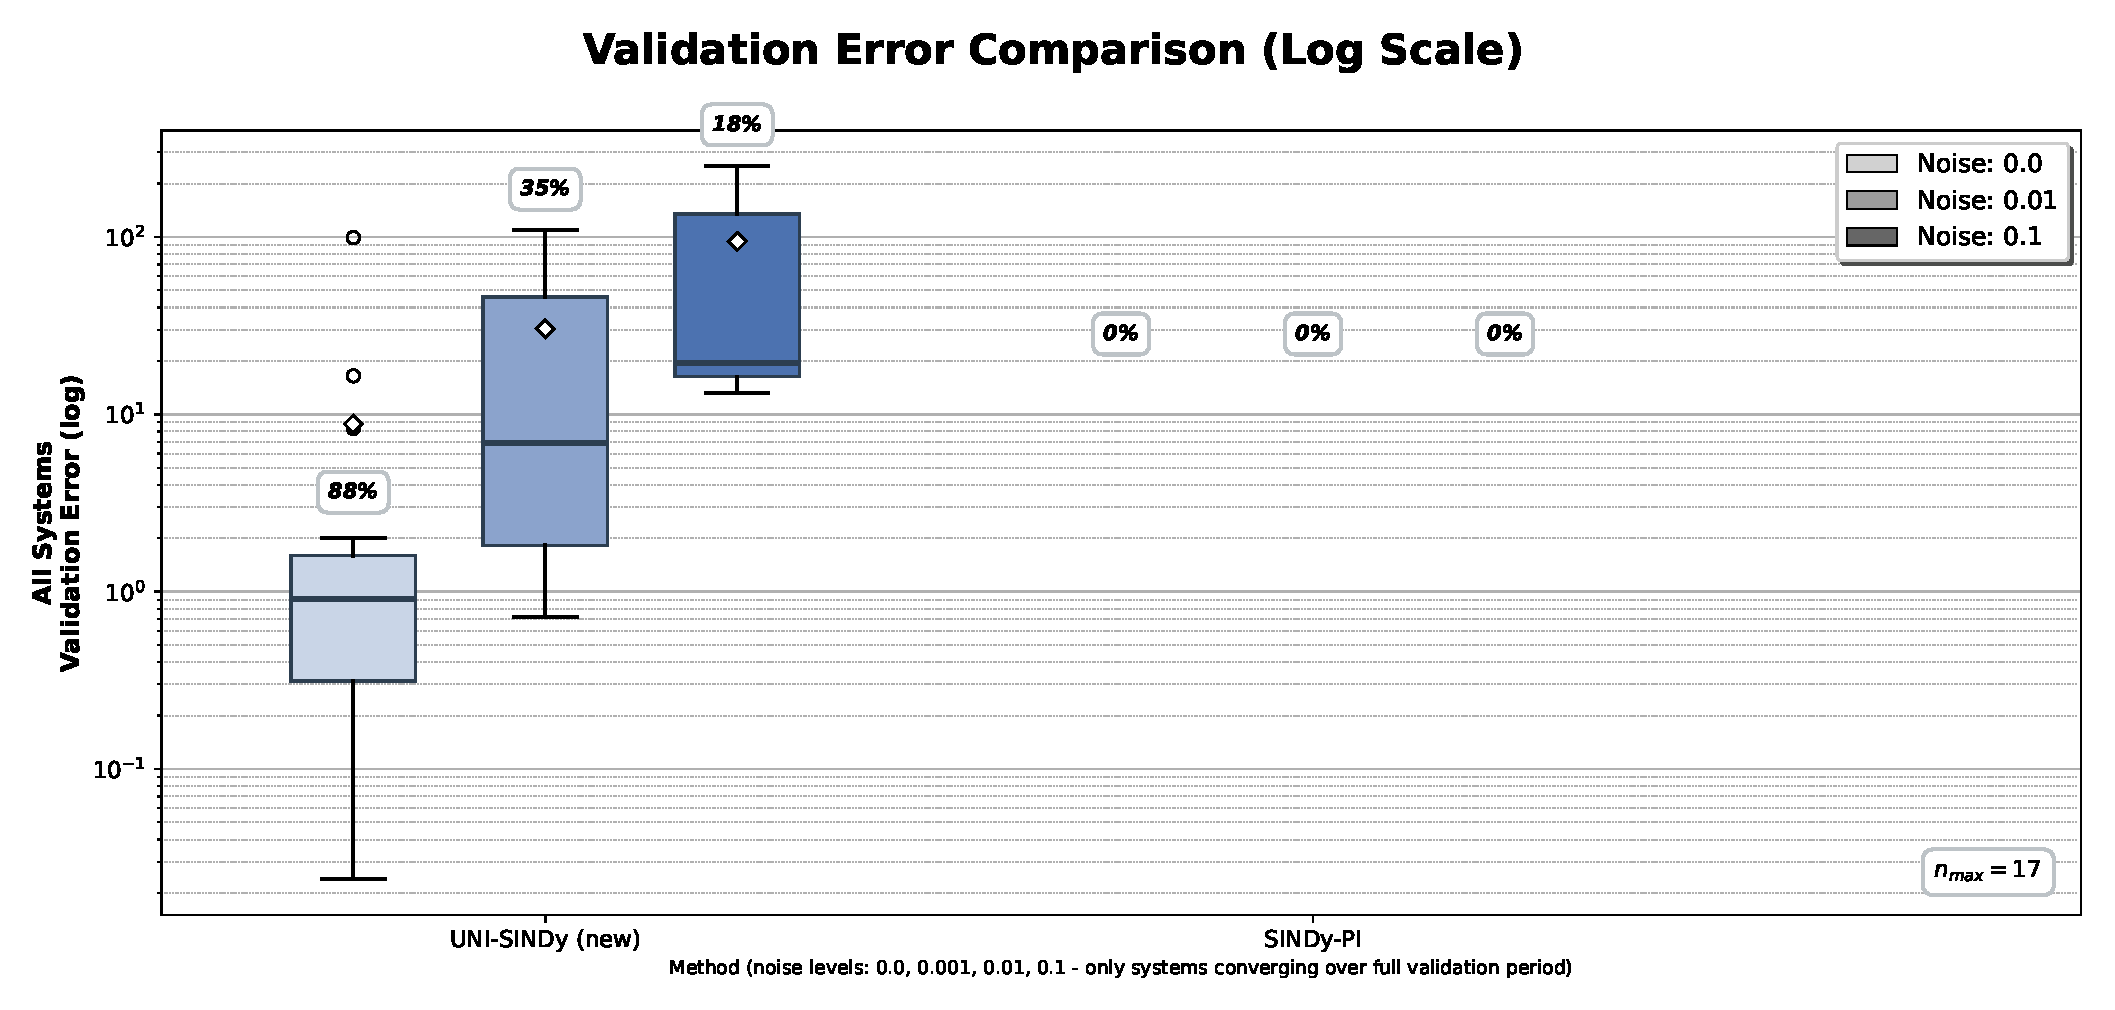
\includegraphics[width=0.95\textwidth]{result/plots_damping_implicit/noise_comparison_combined_white_background.eps}
    
    \vspace{0.5cm}
    
    \includegraphics[width=0.95\textwidth]{result/plots_damping_implicit/success_rate_combined_white_background.eps}
    
    \caption{\textbf{Any damping implicit results:} validation error comparison (top) and success rate comparison (bottom) across all systems}
    \label{fig:damping-implicit}
\end{figure}

\subsection{Any damping mixed experiment}

This subset regroup all the experiment done, there is implicit, explicit, no-damping, damping and add the mixed implicit,explicit experiment.

This is the most meaningfull result of our study because it emphasyze the real robotic system behavior which have passive and active joint. As we can see Fig.~\ref{fig:damping-mixed}, UNI-SINDy is a clear winner in this category in term of successrate. Concerning overall accuracy all methods are on par (likely because when they succeed they show the same amount of performance). UNI-SINDy is also the only one to still discover dynamics on the harder 3-dof system the double pendulum on cartpole. Since UNI-SINDy has been developped to tackle implicit explicit experiment while using the tinyest catalog it is the clear winner in this broad category. This category have all the experiment (192 experiments) which lead to a percentage of discarded experiment of $61\%$. This percentage is the highest among the other category and greatly comes from the fact that mixed experiment from the cartpole double are bigger (due to the 3dof nature that lead to more implicit explicit forces combinaison possible). If we split the percentage discarded experiment along different system we have the following : 
\begin{itemize}
    \item \textbf{Cartpole} : $35\%$ discarded experiment (17/48)
    \item \textbf{Cartpole double} : $79\%$ discarded experiment (76/96)
    \item \textbf{Double pendulum} : $50\%$ discarded experiment (24/48)
\end{itemize}

\begin{figure}[H]
    \centering
    \includegraphics[width=0.95\textwidth]{result/plots_damping_mixed/noise_comparison_combined_white_background.eps}
    
    \vspace{0.5cm}
    
    \includegraphics[width=0.95\textwidth]{result/plots_damping_mixed/success_rate_combined_white_background.eps}
    
    \caption{\textbf{Any damping implicit results:} validation error comparison (top) and success rate comparison (bottom) across all systems}
    \label{fig:damping-mixed}
\end{figure}

% -------------------------------------------------------------------------
%   BACK MATTER
% -------------------------------------------------------------------------

\printbibliography

\appendix
\chapter{Python Implementation}

\begin{lstlisting}[language=Python, caption={\textbf{Weak sparsity function}}, label=lst:weak-sparsity]
def _weak_sparsity_rank_weighted(x):

    x = np.abs(x)
    s = np.sort(x)[::-1] # descending order
    ranks = np.arange(1, len(s) + 1)

    weights = 1.0 / ranks
    weighted_sum = np.sum(s * weights)
    weight_total = np.sum(s)

    if weight_total == 0:
        return 0
    else:
        return weighted_sum / weight_total

\end{lstlisting}

\chapter{All data figures}
\label{ch:all-result-figures}

\section{Damping Explicit Results}

\begin{figure}[H]
    \centering
    \begin{subfigure}[b]{0.95\textwidth}
        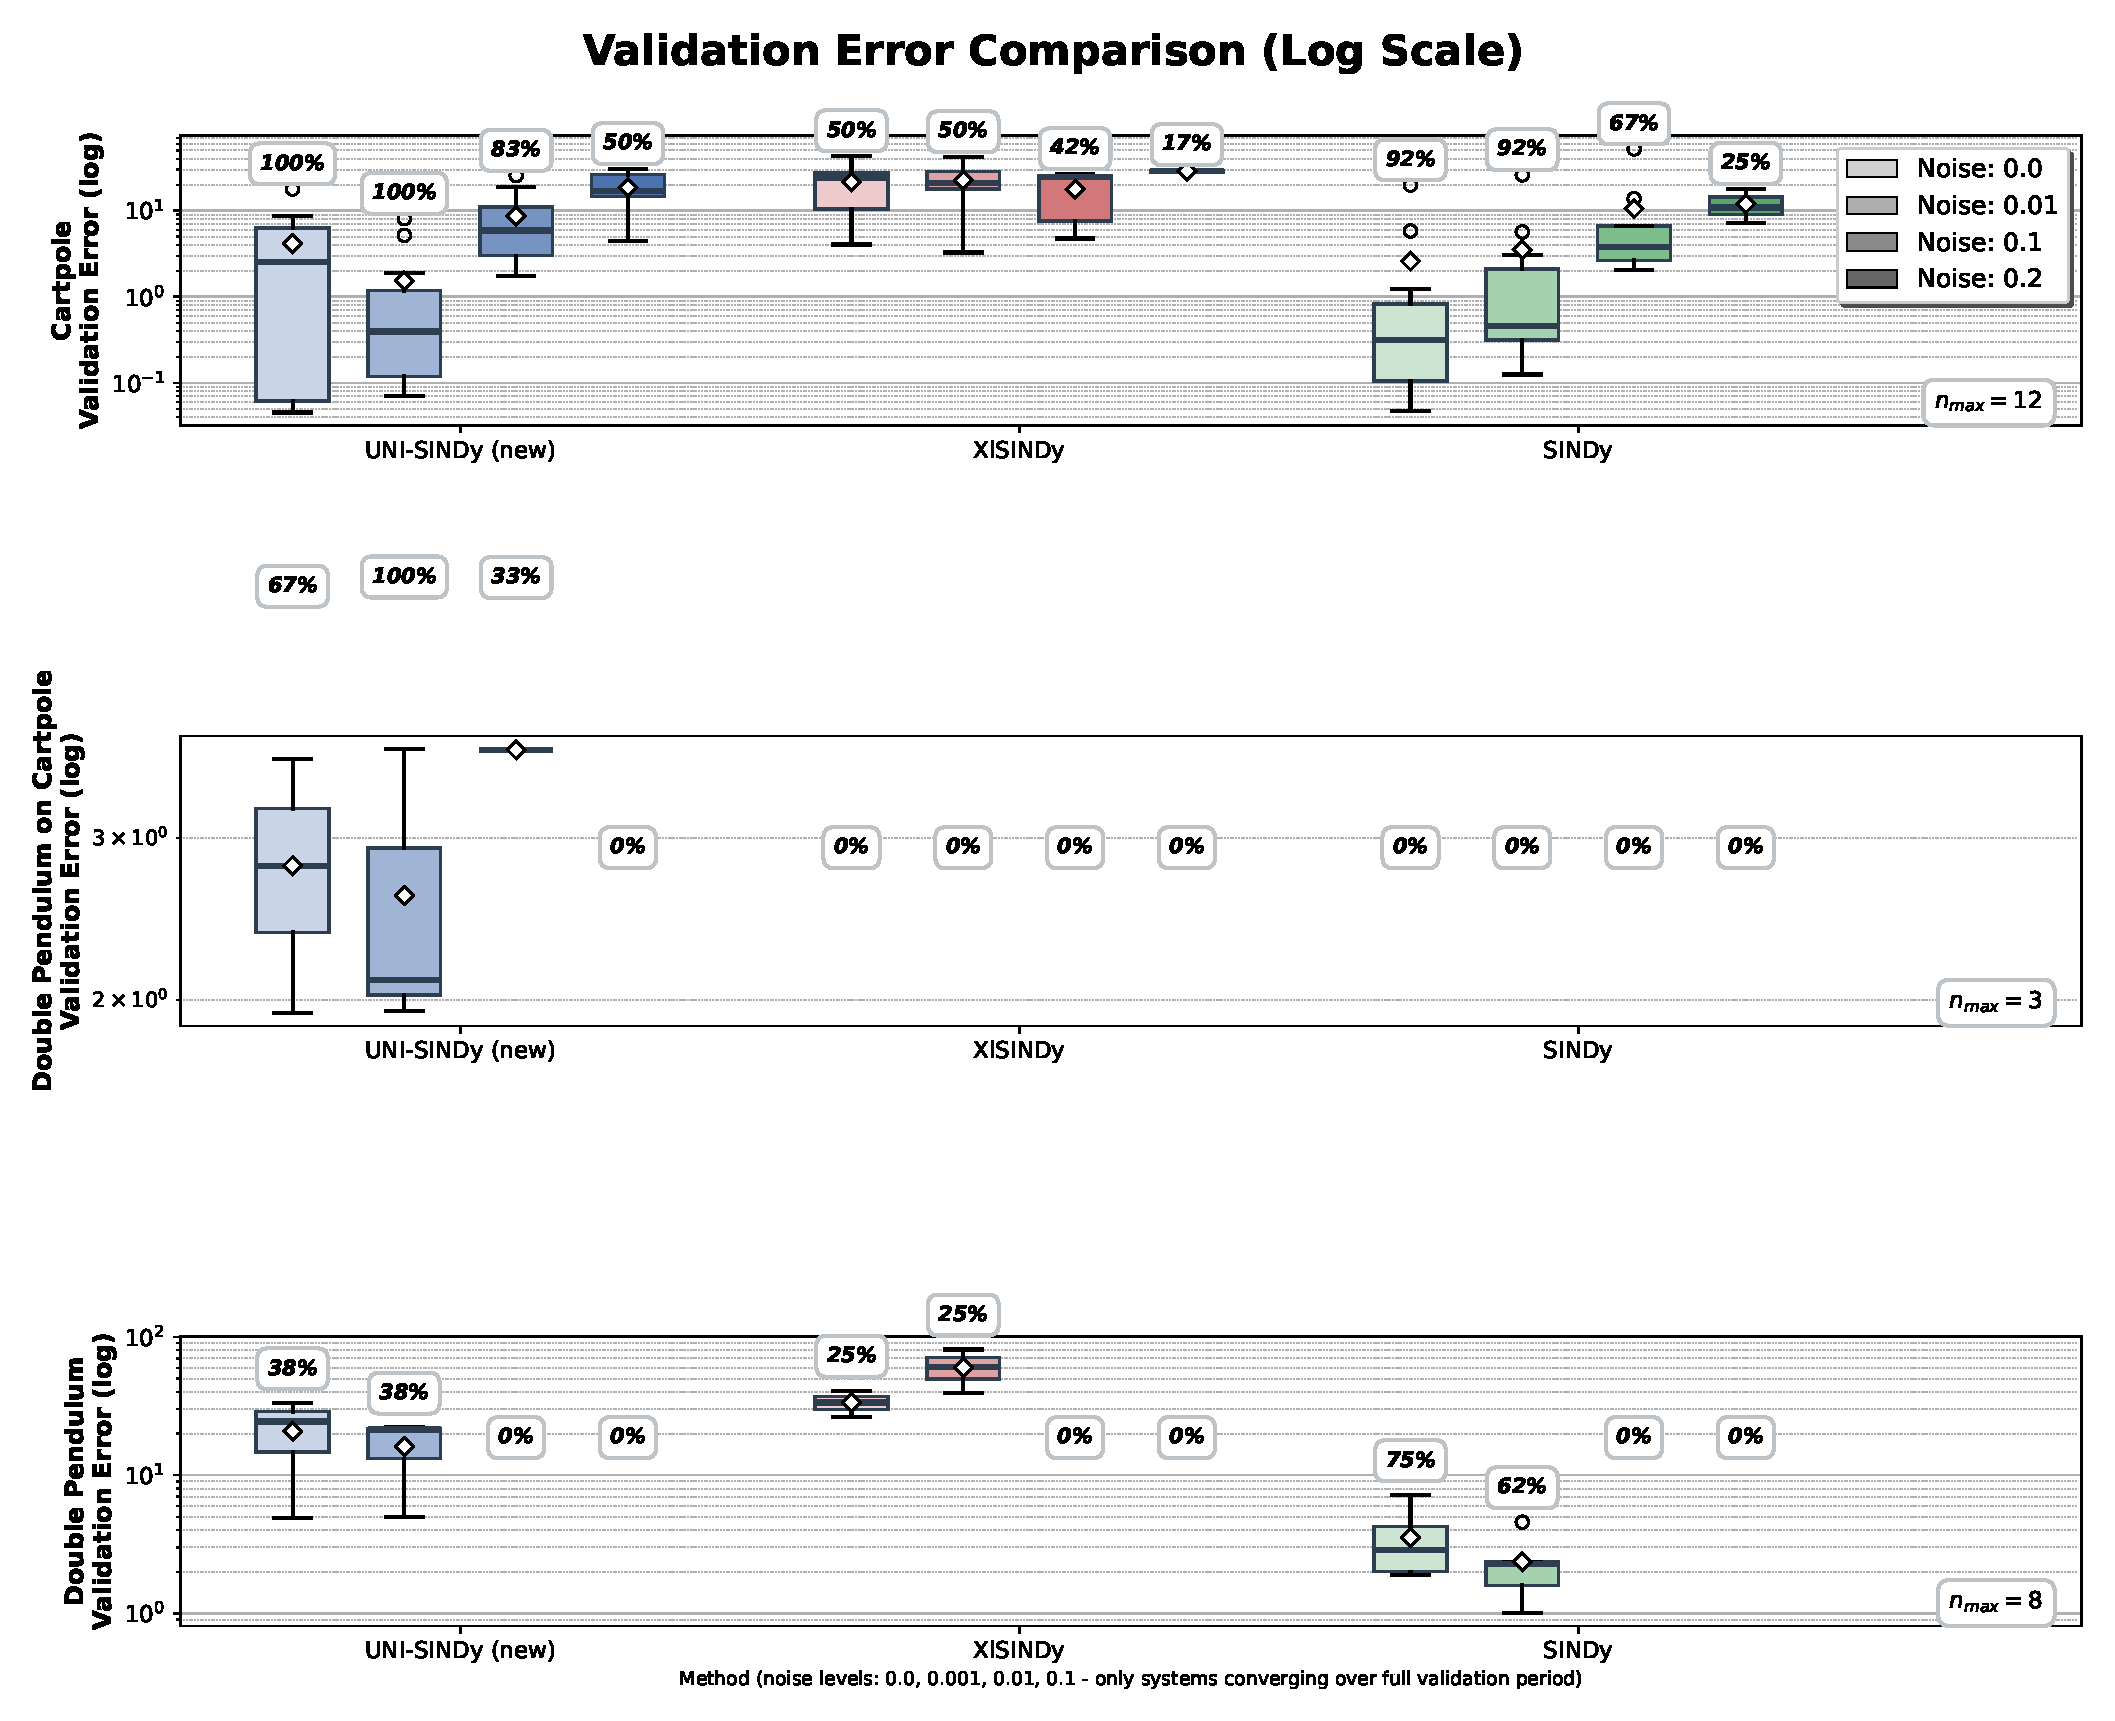
\includegraphics[width=\textwidth]{result/plots_damping_explicit/noise_comparison_white_background.eps}
        \caption{Noise comparison}
    \end{subfigure}
    
    \vspace{0.5cm}
    
    \begin{subfigure}[b]{0.95\textwidth}
        \includegraphics[width=\textwidth]{result/plots_damping_explicit/noise_comparison_combined_white_background.eps}
        \caption{Noise comparison combined}
    \end{subfigure}
    \caption{Damping explicit - Validation error comparison}
    \label{fig:damping_explicit_validation}
\end{figure}

\begin{figure}[H]
    \centering
    \begin{subfigure}[b]{0.95\textwidth}
        \includegraphics[width=\textwidth]{result/plots_damping_explicit/success_rate_white_background.eps}
        \caption{Success rate}
    \end{subfigure}
    
    \vspace{0.5cm}
    
    \begin{subfigure}[b]{0.95\textwidth}
        \includegraphics[width=\textwidth]{result/plots_damping_explicit/success_rate_combined_white_background.eps}
        \caption{Success rate combined}
    \end{subfigure}
    \caption{Damping explicit - Success rate comparison}
    \label{fig:damping_explicit_success}
\end{figure}

\section{Damping Implicit Results}

\begin{figure}[H]
    \centering
    \begin{subfigure}[b]{0.95\textwidth}
        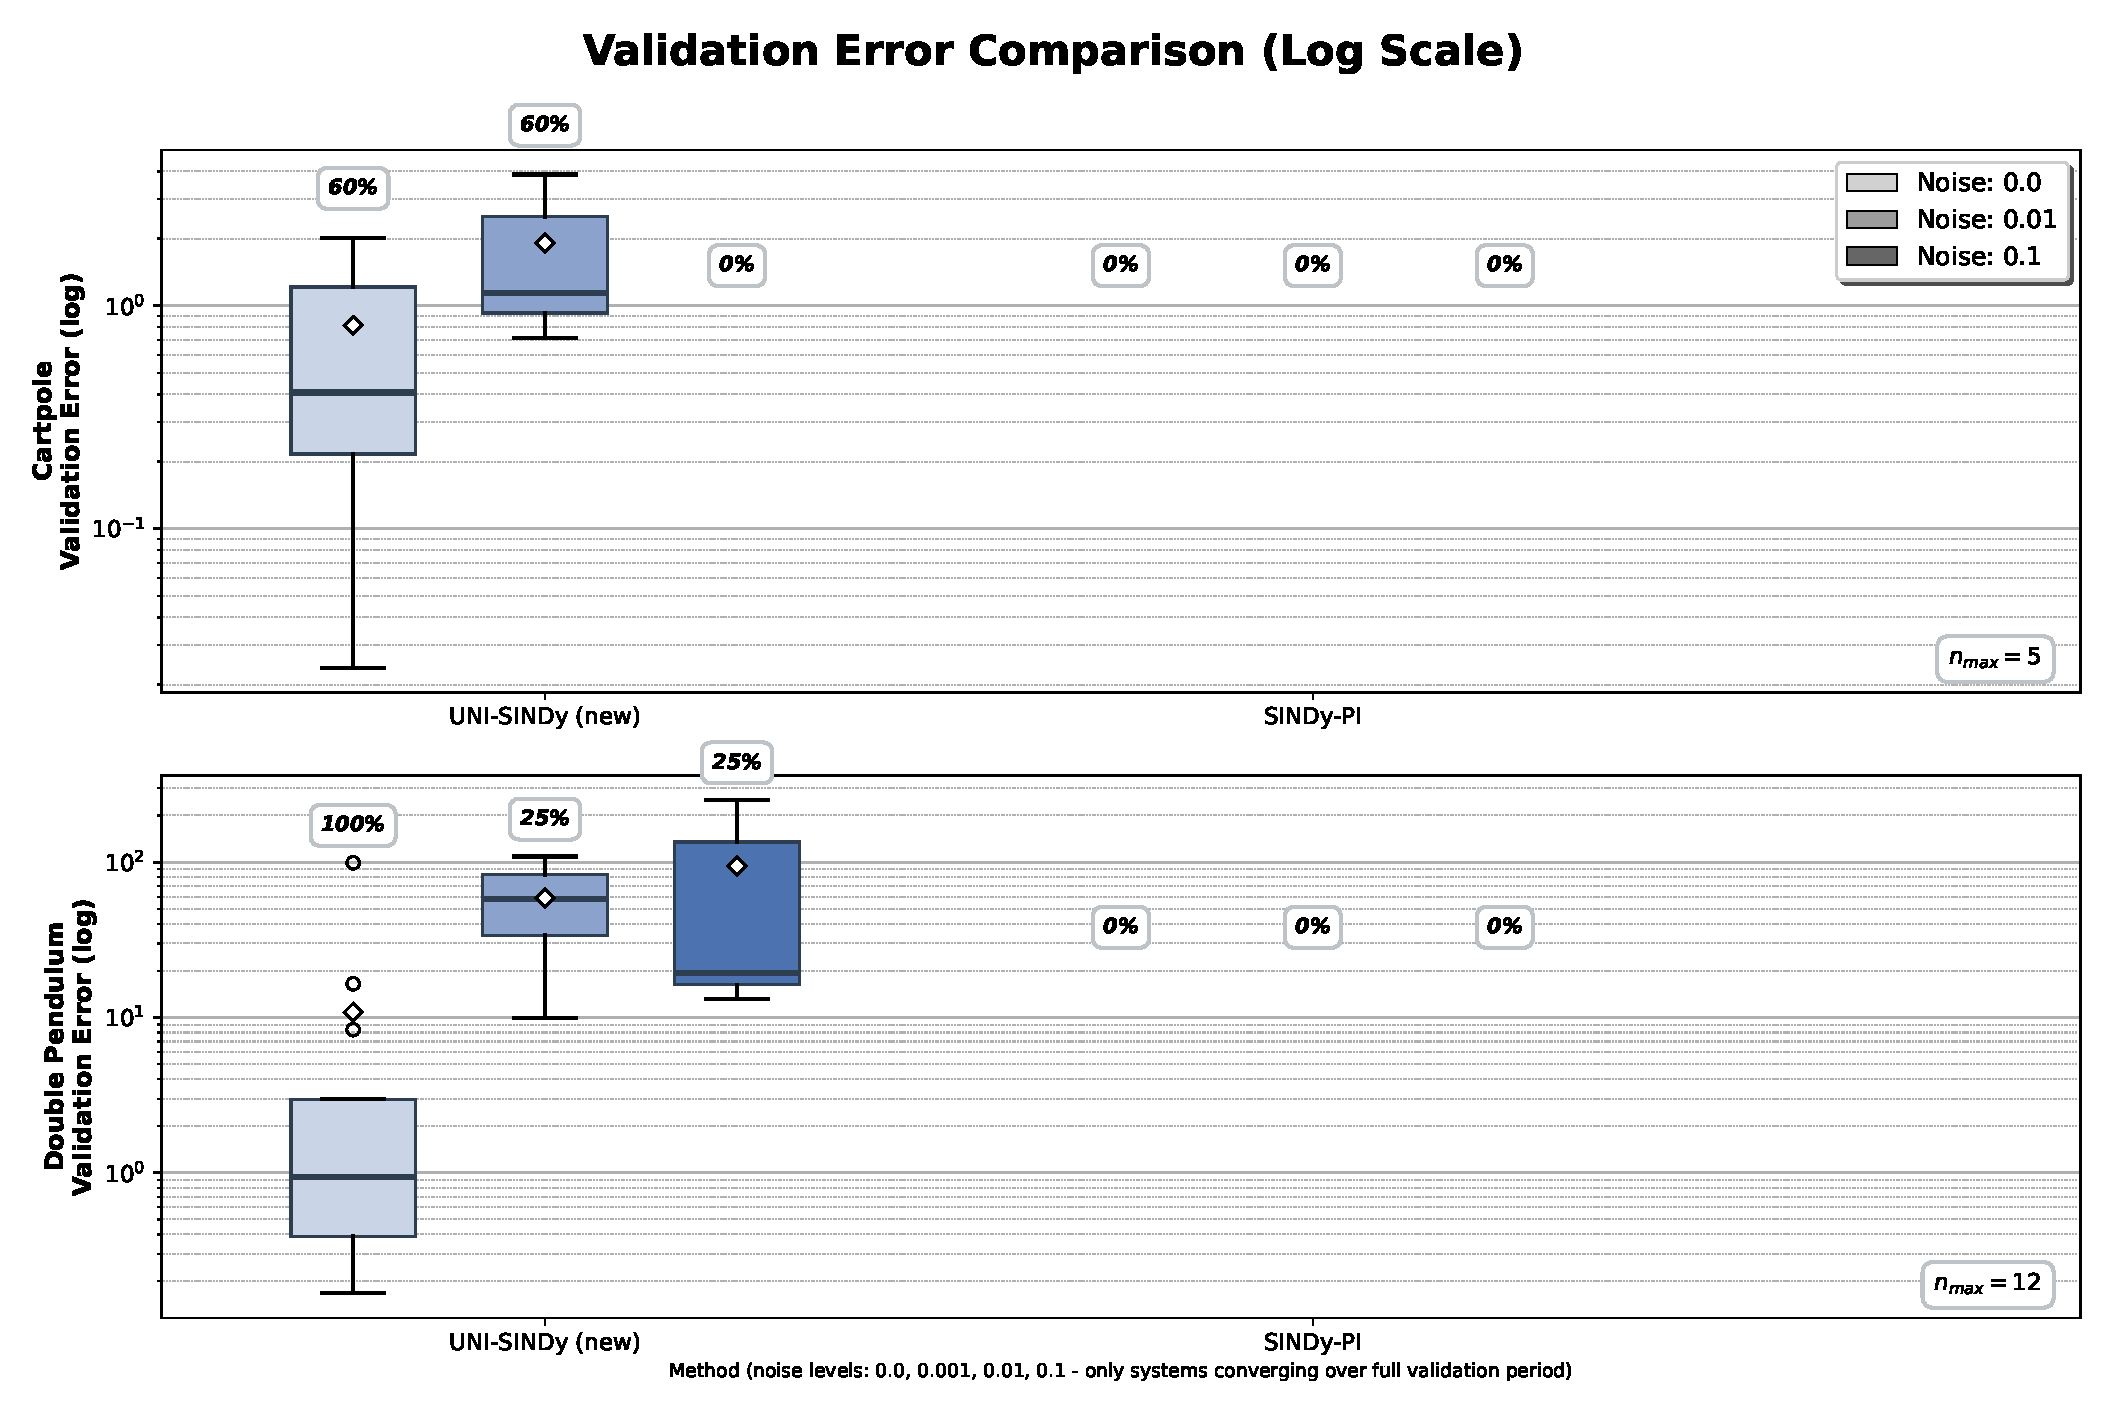
\includegraphics[width=\textwidth]{result/plots_damping_implicit/noise_comparison_white_background.eps}
        \caption{Noise comparison}
    \end{subfigure}
    
    \vspace{0.5cm}
    
    \begin{subfigure}[b]{0.95\textwidth}
        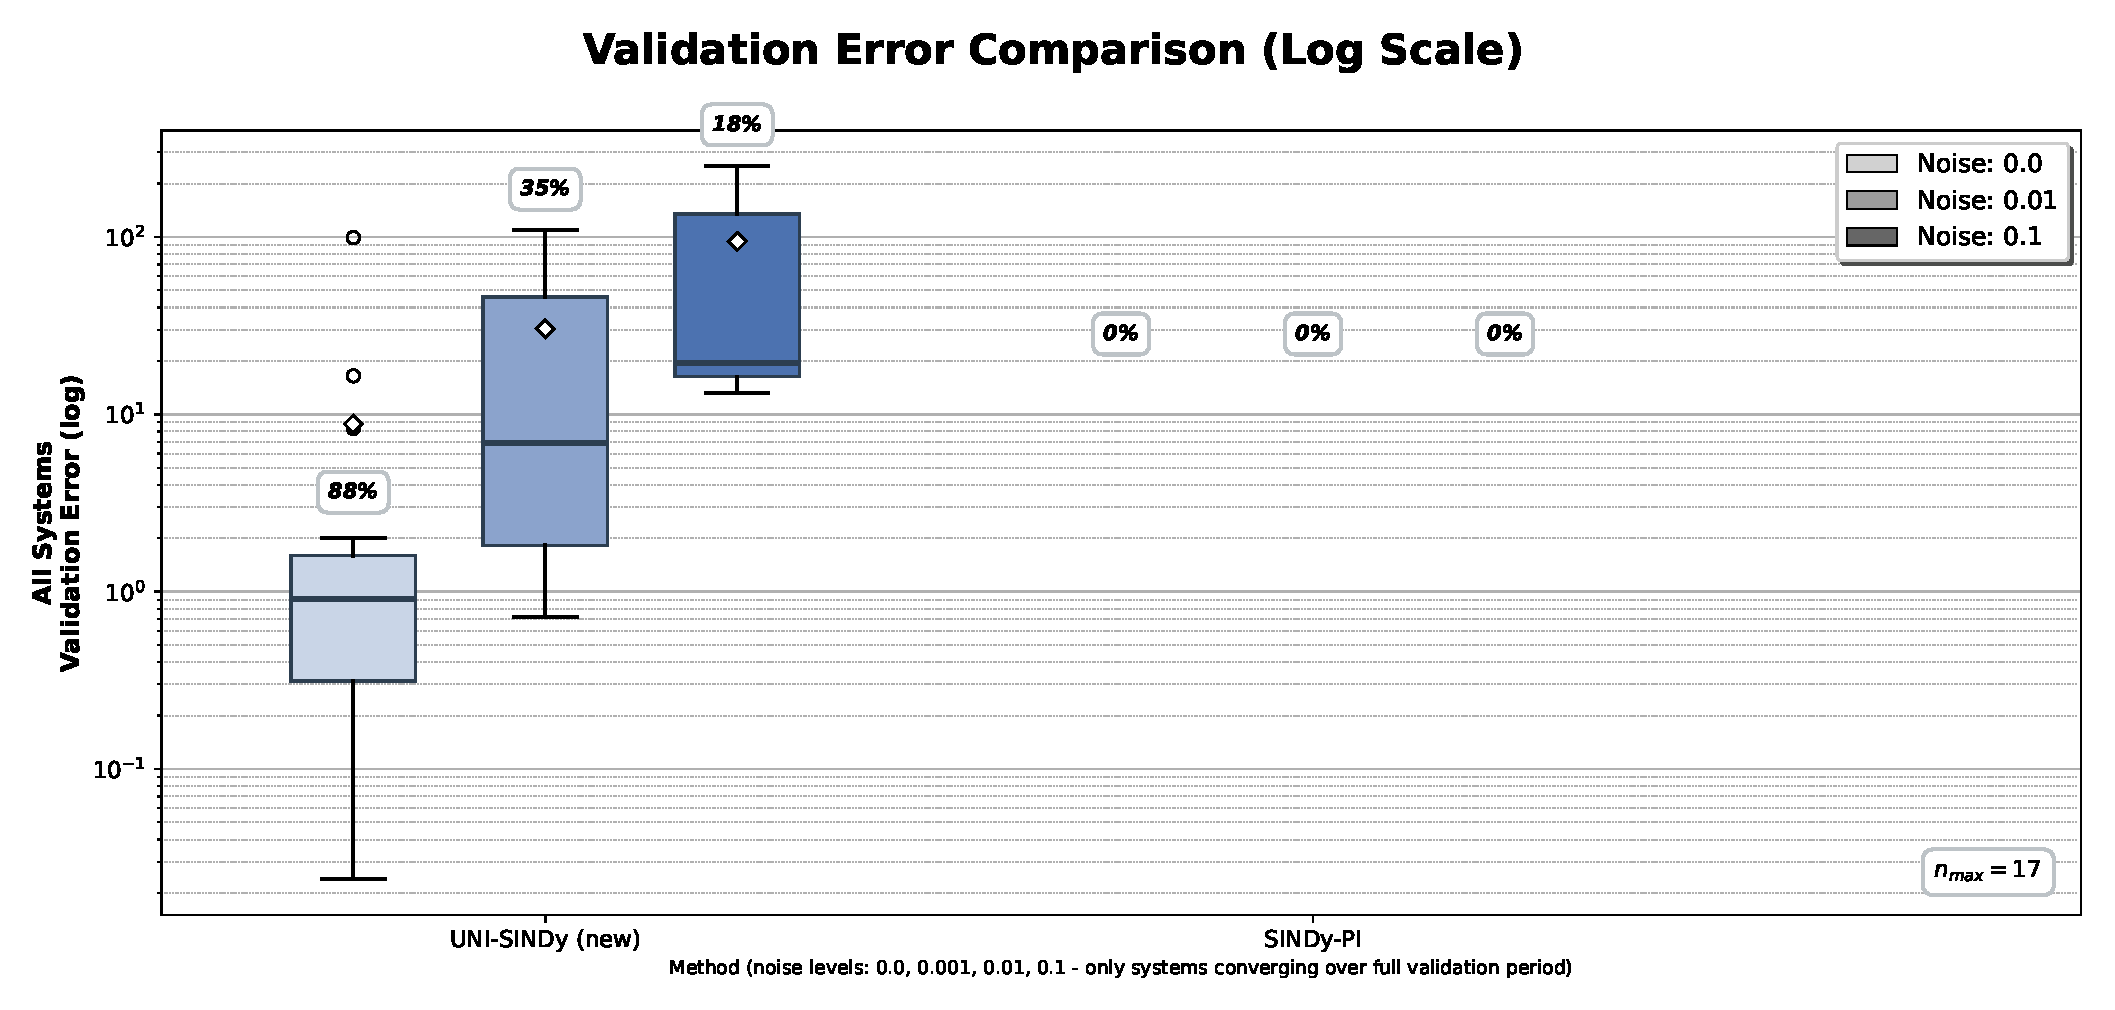
\includegraphics[width=\textwidth]{result/plots_damping_implicit/noise_comparison_combined_white_background.eps}
        \caption{Noise comparison combined}
    \end{subfigure}
    \caption{Damping implicit - Validation error comparison}
    \label{fig:damping_implicit_validation}
\end{figure}

\begin{figure}[H]
    \centering
    \begin{subfigure}[b]{0.95\textwidth}
        \includegraphics[width=\textwidth]{result/plots_damping_implicit/success_rate_white_background.eps}
        \caption{Success rate}
    \end{subfigure}
    
    \vspace{0.5cm}
    
    \begin{subfigure}[b]{0.95\textwidth}
        \includegraphics[width=\textwidth]{result/plots_damping_implicit/success_rate_combined_white_background.eps}
        \caption{Success rate combined}
    \end{subfigure}
    \caption{Damping implicit - Success rate comparison}
    \label{fig:damping_implicit_success}
\end{figure}

\section{Damping Mixed Results}

\begin{figure}[H]
    \centering
    \begin{subfigure}[b]{0.95\textwidth}
        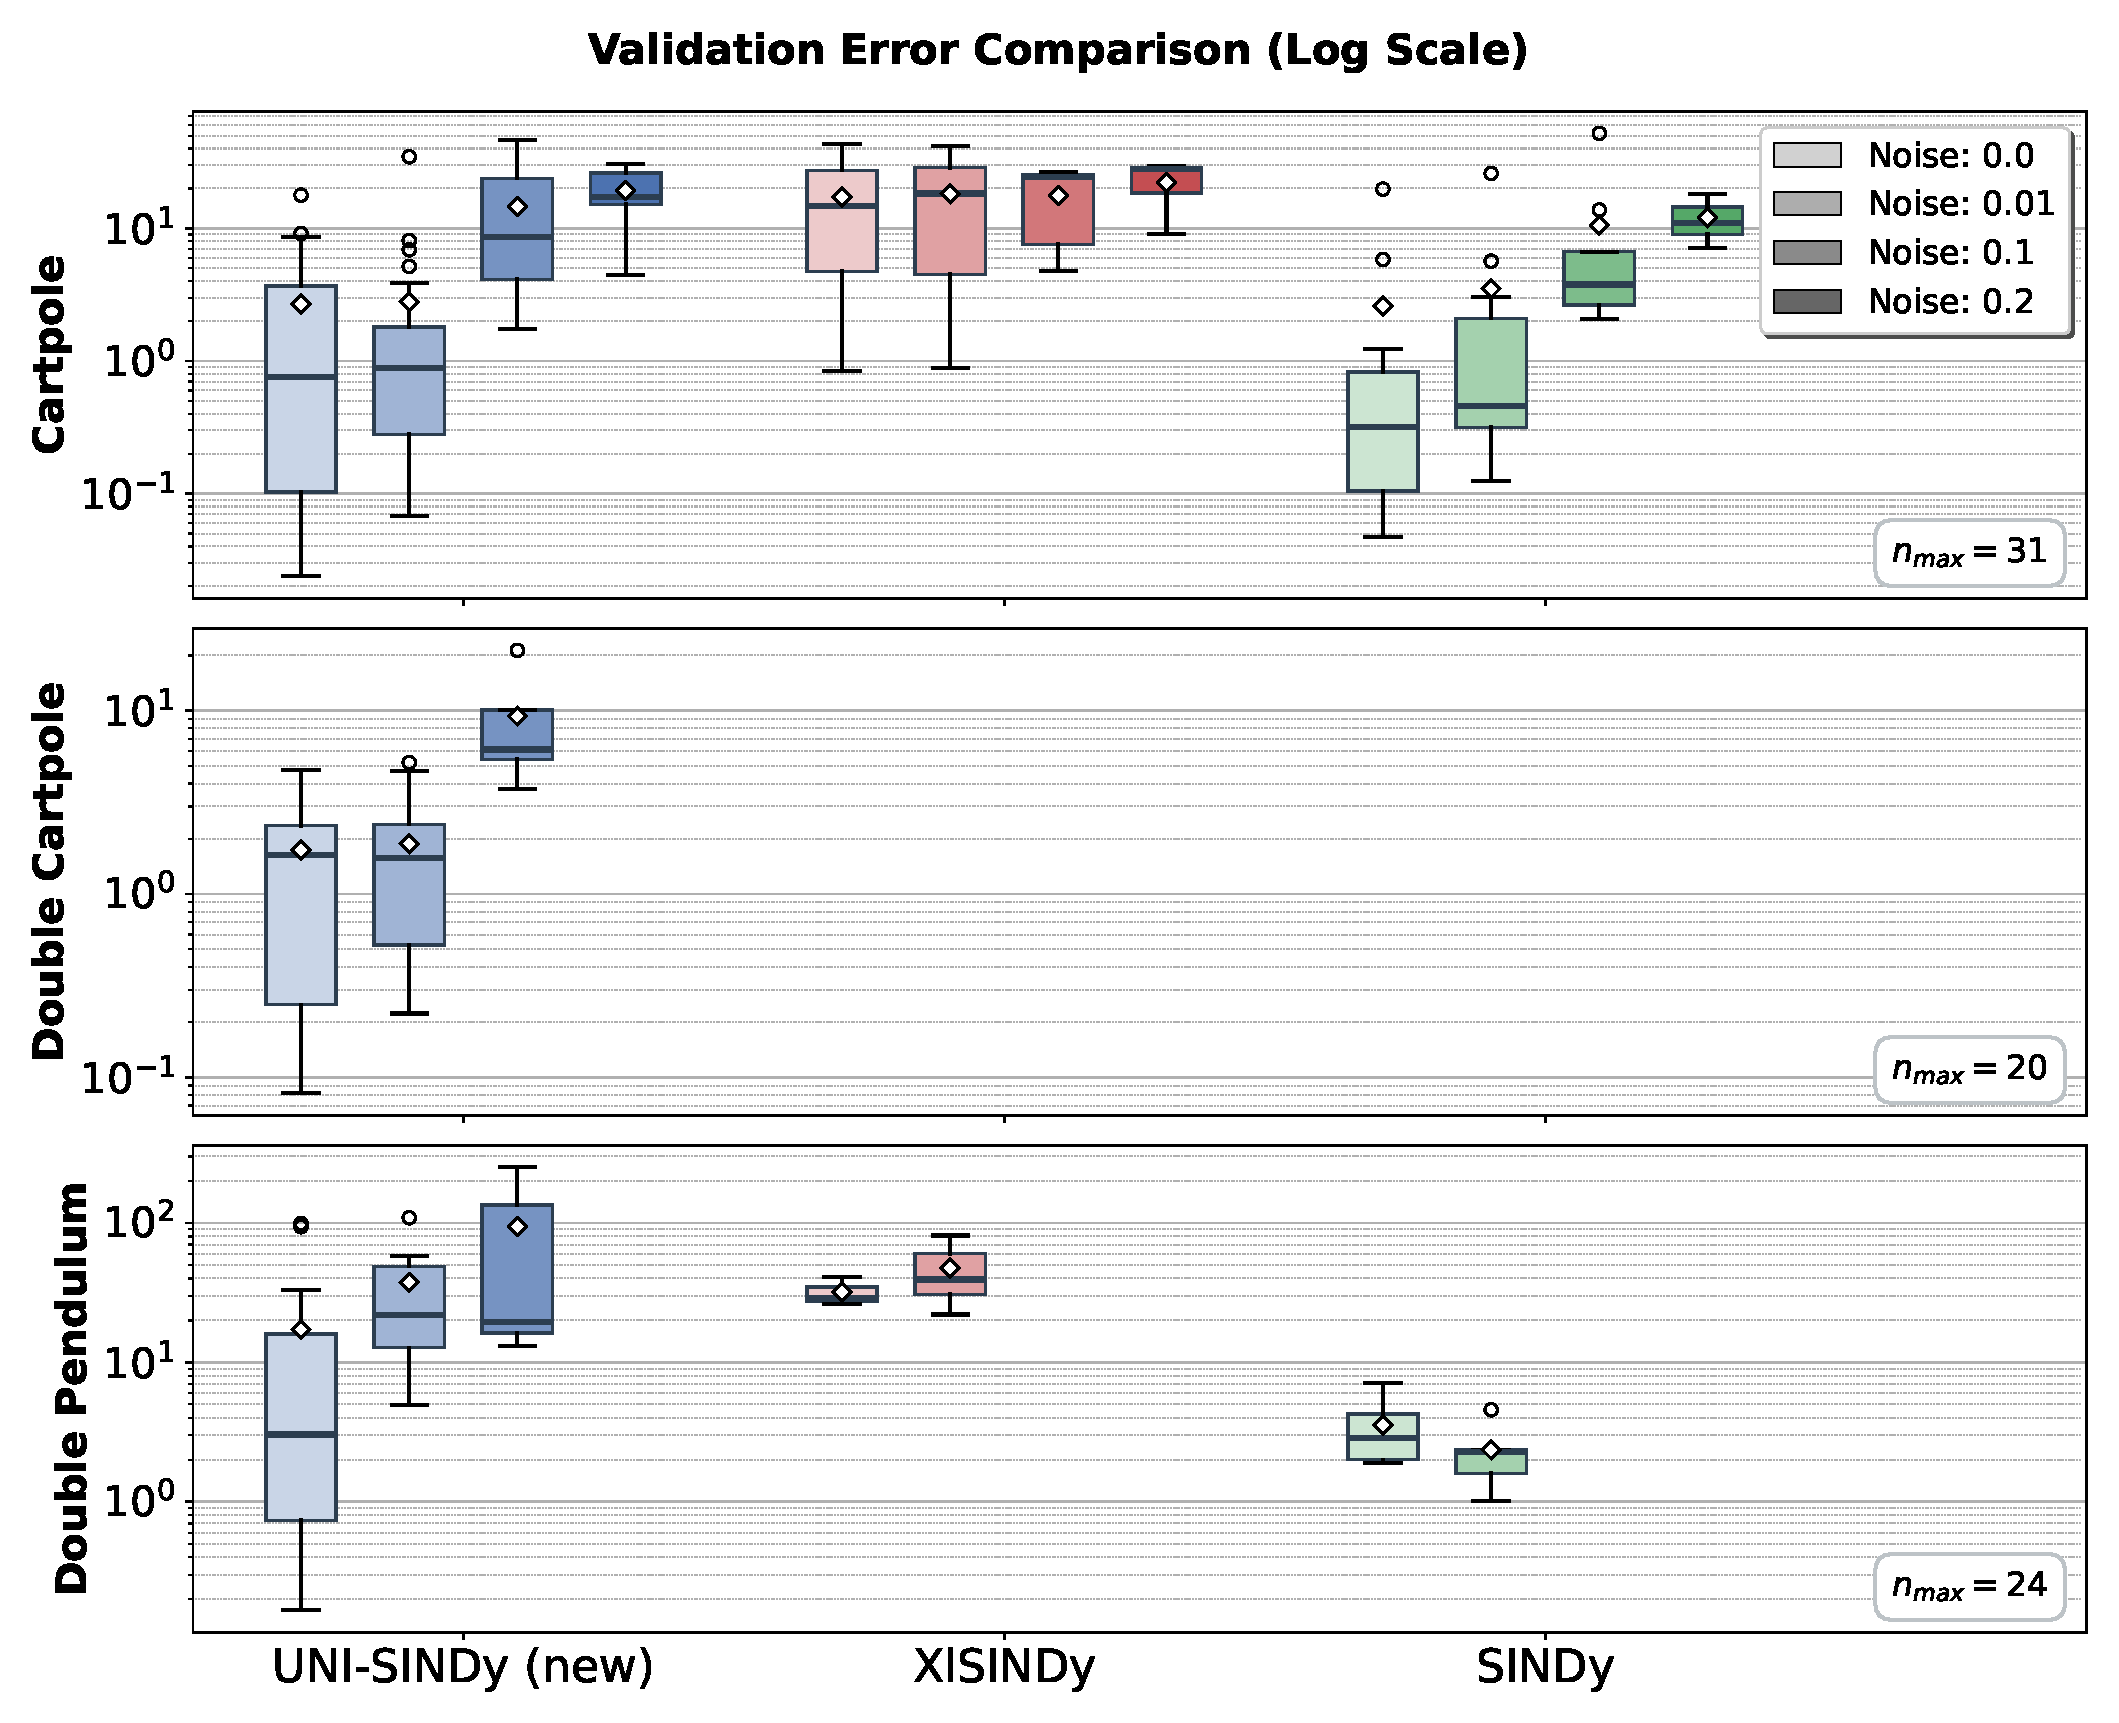
\includegraphics[width=\textwidth]{result/plots_damping_mixed/noise_comparison_white_background.eps}
        \caption{Noise comparison}
    \end{subfigure}
    
    \vspace{0.5cm}
    
    \begin{subfigure}[b]{0.95\textwidth}
        \includegraphics[width=\textwidth]{result/plots_damping_mixed/noise_comparison_combined_white_background.eps}
        \caption{Noise comparison combined}
    \end{subfigure}
    \caption{Damping mixed - Validation error comparison}
    \label{fig:damping_mixed_validation}
\end{figure}

\begin{figure}[H]
    \centering
    \begin{subfigure}[b]{0.95\textwidth}
        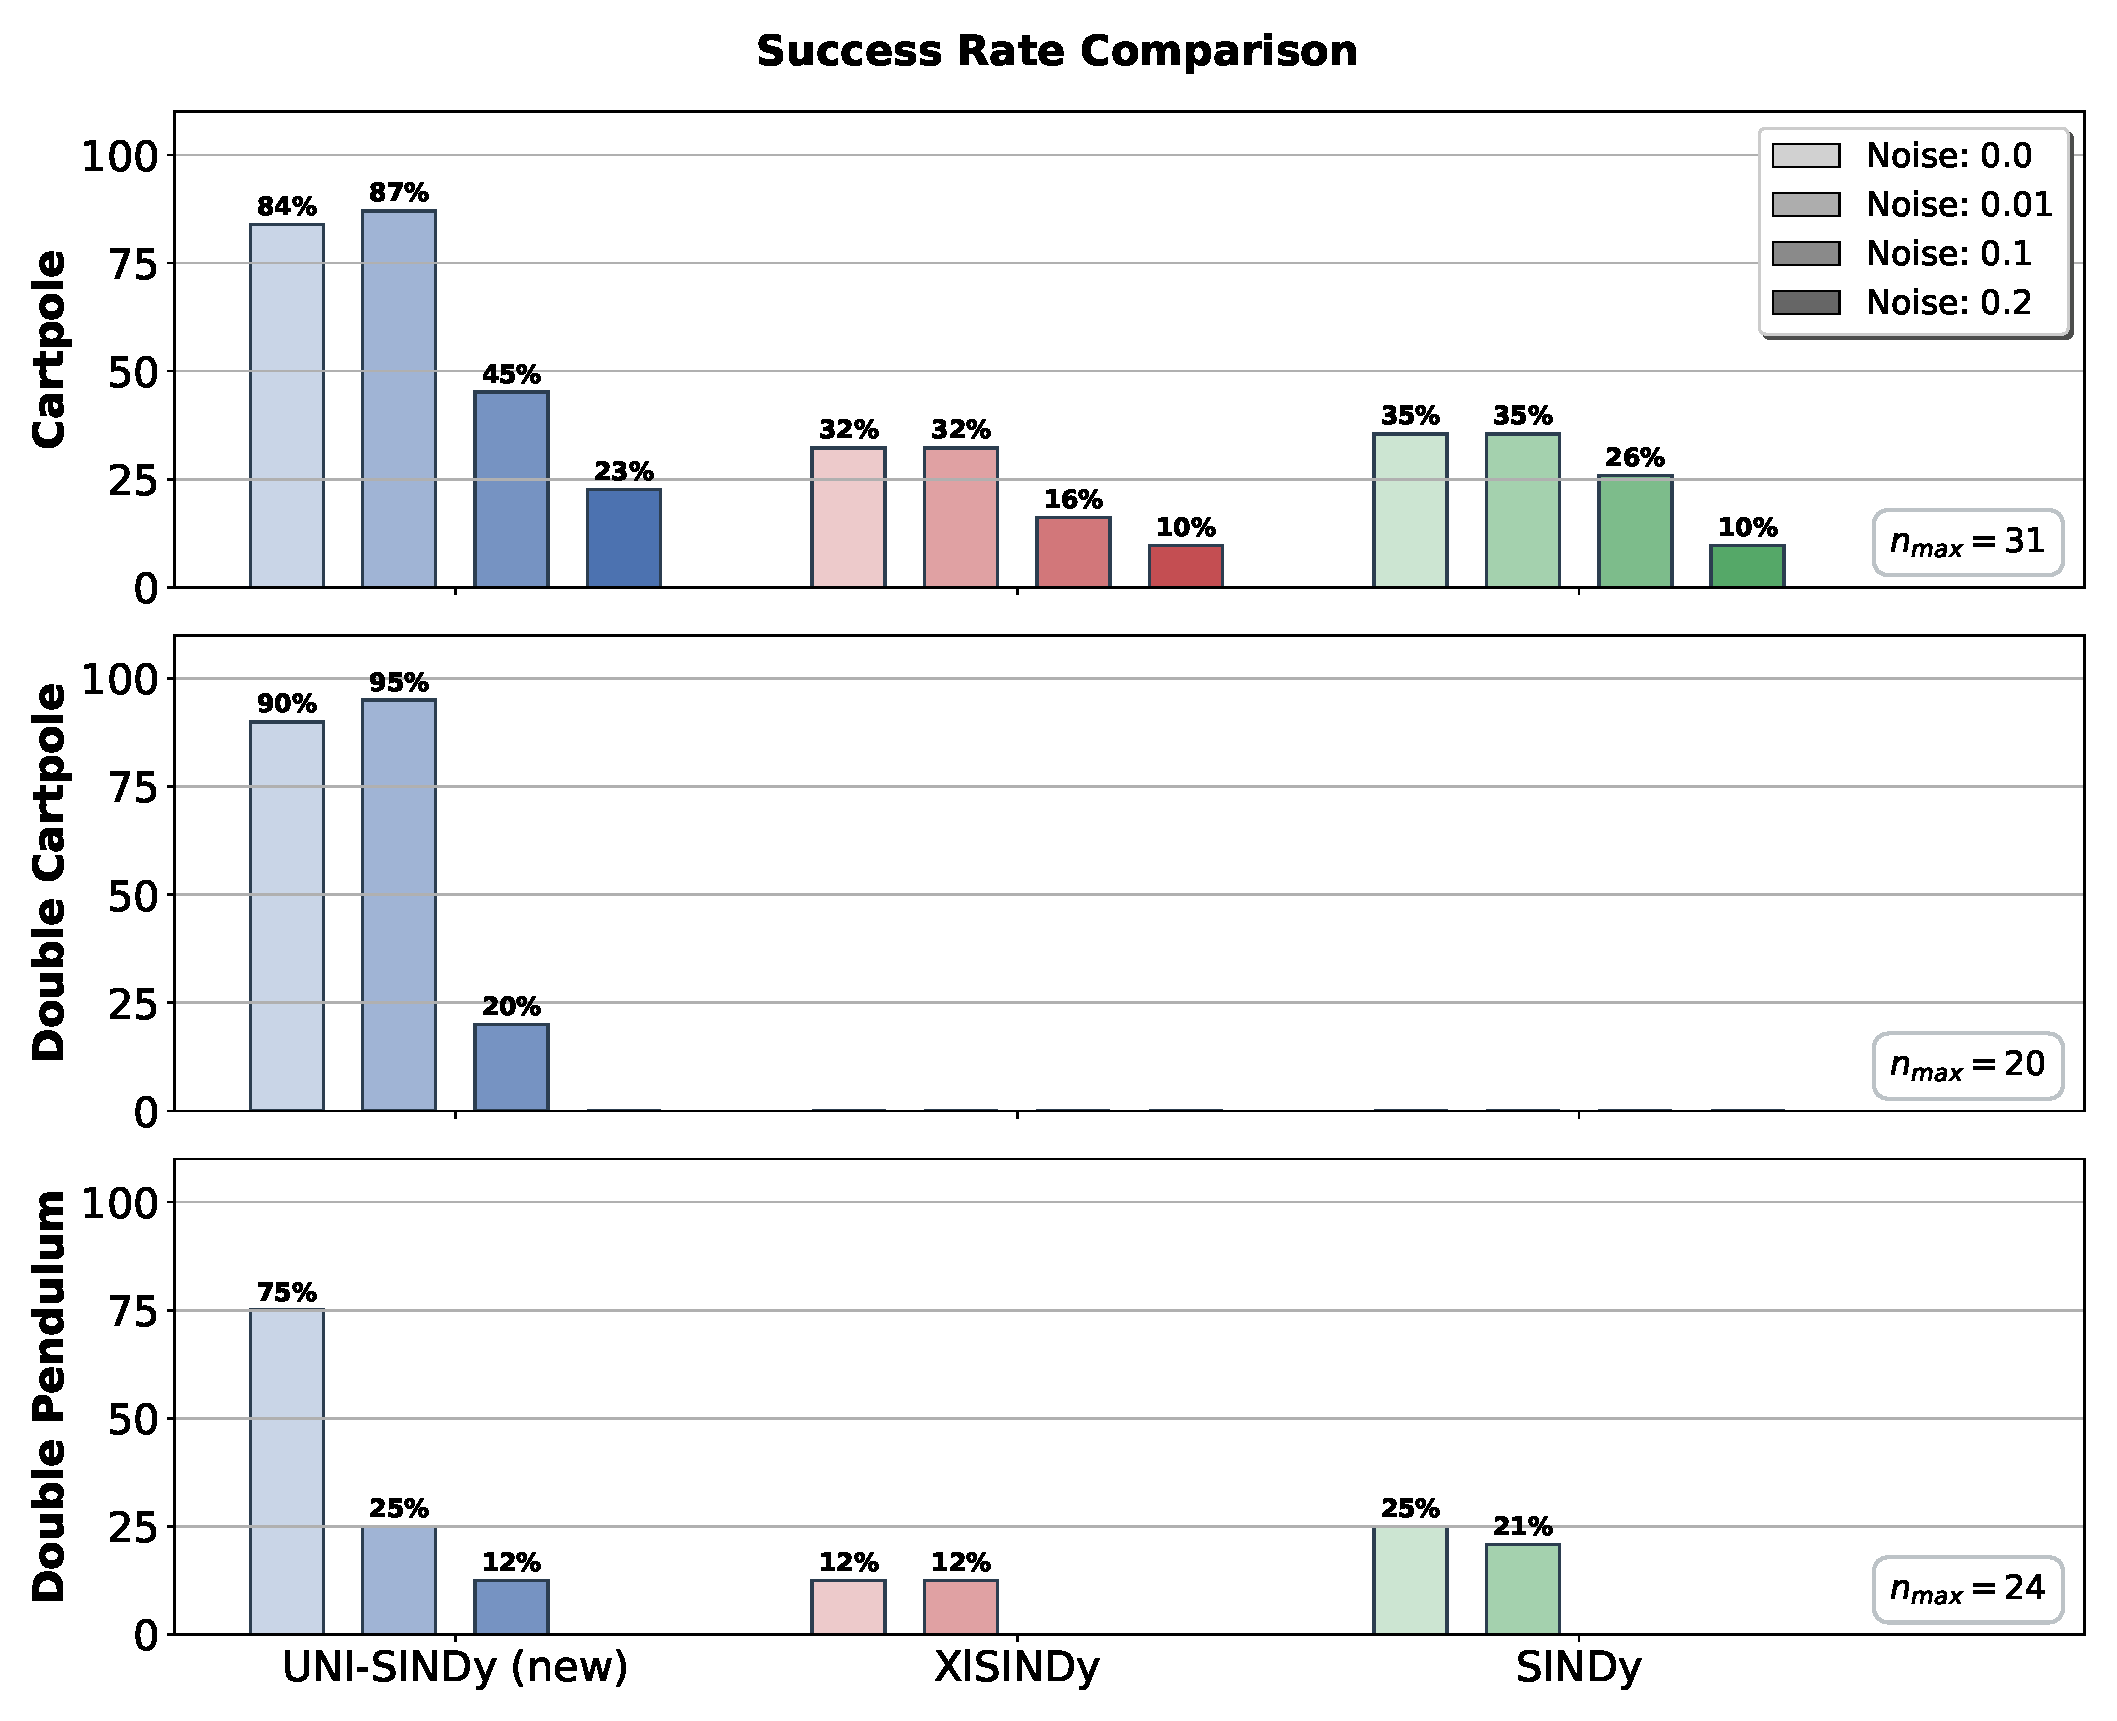
\includegraphics[width=\textwidth]{result/plots_damping_mixed/success_rate_white_background.eps}
        \caption{Success rate}
    \end{subfigure}
    
    \vspace{0.5cm}
    
    \begin{subfigure}[b]{0.95\textwidth}
        \includegraphics[width=\textwidth]{result/plots_damping_mixed/success_rate_combined_white_background.eps}
        \caption{Success rate combined}
    \end{subfigure}
    \caption{Damping mixed - Success rate comparison}
    \label{fig:damping_mixed_success}
\end{figure}

\section{No Damping Explicit Results}

\begin{figure}[H]
    \centering
    \begin{subfigure}[b]{0.95\textwidth}
        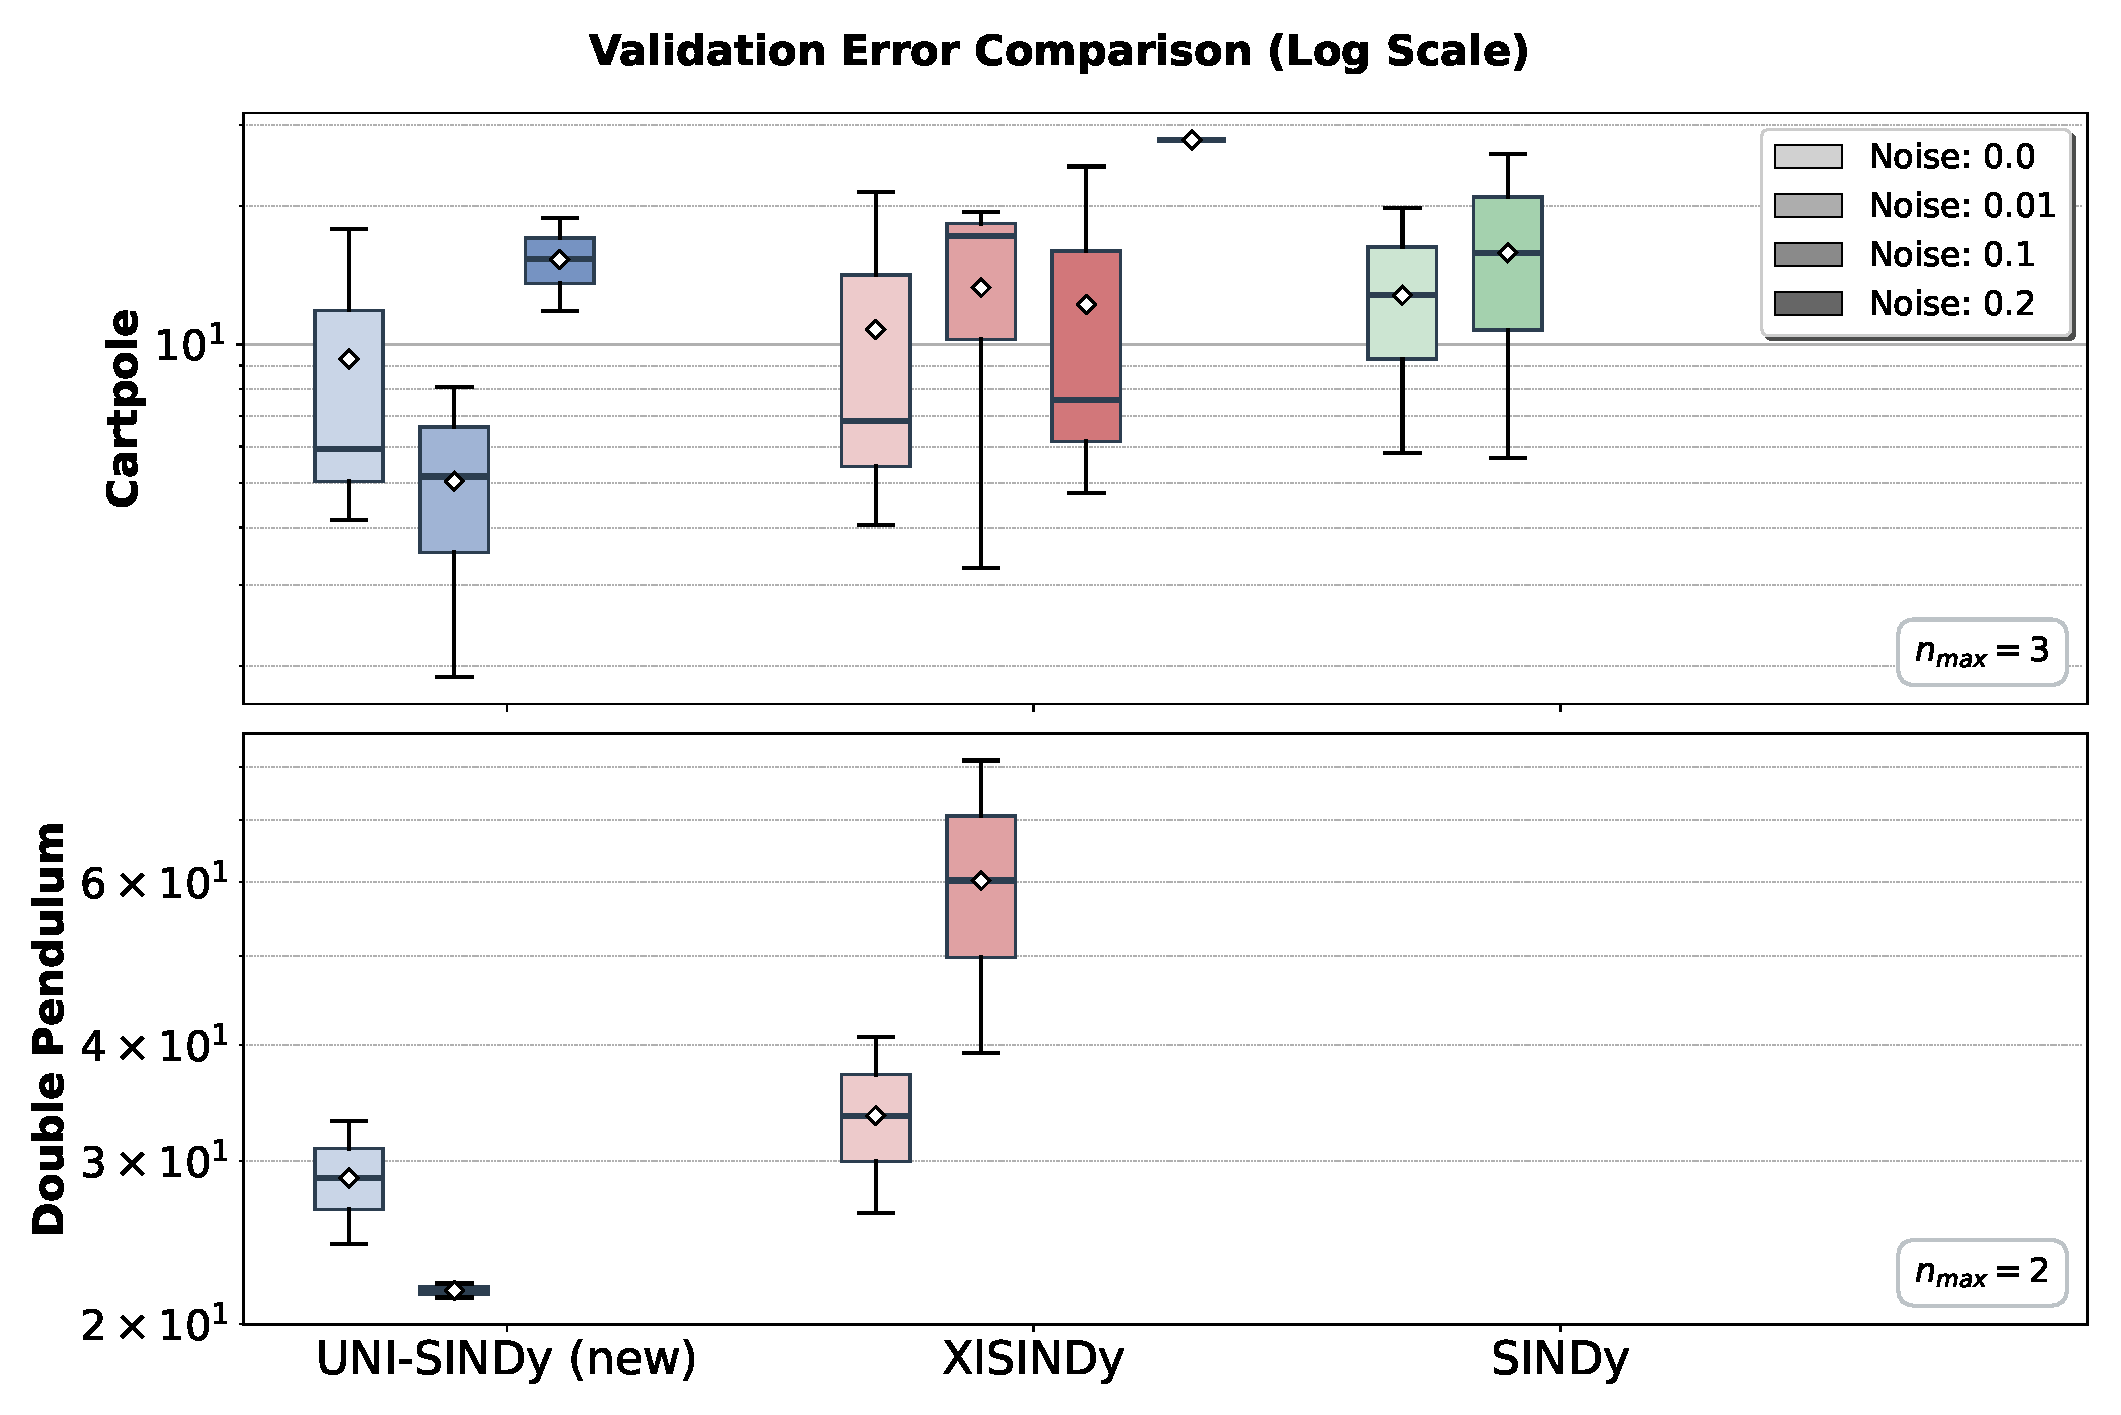
\includegraphics[width=\textwidth]{result/plots_no_damping_explicit/noise_comparison_white_background.eps}
        \caption{Noise comparison}
    \end{subfigure}
    
    \vspace{0.5cm}
    
    \begin{subfigure}[b]{0.95\textwidth}
        \includegraphics[width=\textwidth]{result/plots_no_damping_explicit/noise_comparison_combined_white_background.eps}
        \caption{Noise comparison combined}
    \end{subfigure}
    \caption{No damping explicit - Validation error comparison}
    \label{fig:no_damping_explicit_validation}
\end{figure}

\begin{figure}[H]
    \centering
    \begin{subfigure}[b]{0.95\textwidth}
        \includegraphics[width=\textwidth]{result/plots_no_damping_explicit/success_rate_white_background.eps}
        \caption{Success rate}
    \end{subfigure}
    
    \vspace{0.5cm}
    
    \begin{subfigure}[b]{0.95\textwidth}
        \includegraphics[width=\textwidth]{result/plots_no_damping_explicit/success_rate_combined_white_background.eps}
        \caption{Success rate combined}
    \end{subfigure}
    \caption{No damping explicit - Success rate comparison}
    \label{fig:no_damping_explicit_success}
\end{figure}

\end{document}